\documentclass[a4paper,12pt, openany]{book}


%%% Работа с русским языком
\usepackage{cmap}          % поиск в PDF
\usepackage[T2A]{fontenc}      % кодировка
\usepackage[utf8]{inputenc}    % кодировка исходного текста
%\usepackage{fixint}
\usepackage[russian]{babel}  % локализация и переносы
%\usepackage{pscyr}
\usepackage{mathtools, nccmath}
%\renewcommand{\rmdefault}{cmss}
%%% Дополнительная работа с математикой
\usepackage{amsmath,amsfonts,amssymb,amsthm,mathtools} % AMS
\usepackage{titlesec}
\titleformat{\section}{\filcenter\rmfamily\Large\bfseries}{\thesection.}{0.2em}{}
\titleformat{\subsection}{\filcenter\rmfamily\large\bfseries}{\thesubsection.}{0.2em}{}
\titleformat{\subsubsection}{\filcenter\rmfamily\large\bfseries}{\thesubsubsection.}{0.2em}{}
%% Номера формул
%\mathtoolsset{showonlyrefs=true} % Показывать номера только у тех формул, на которые есть \eqref{} в тексте.
%\usepackage{leqno} % Нумерация формул слева
%\usepackage{rumathgrk1}
%\usepackage{MnSymbol}
%% Перенос знаков в формулах (по Львовскому)
\newcommand{\hm}[1]{#1\nobreak\discretionary{}{\hbox{\ensuremath{#1}}}{}}
%\usepackage{glonti}
%%% Работа с картинками
\usepackage{graphicx}  % Для вставки рисунков

\graphicspath{{images/}}  % папки с картинками
\usepackage{wrapfig} % Обтекание рисунков текстом
\addto\captionsrussian{\def\refname{Список используемой литературы}}
%%% Работа с таблицами
\usepackage{array,tabularx,tabulary} % Дополнительная работа с таблицами
\usepackage{longtable}  % Длинные таблицы
\usepackage{multirow} % Слияние строк в таблице
%%% Теоремы
\theoremstyle{plain} % Это стиль по умолчанию, его можно не переопределять.
\newtheorem{theorem}{Теорема}[section]
\newtheorem{proposition}[theorem]{Утверждение}
\usepackage{subcaption}
\theoremstyle{definition} % "Определение"
\newtheorem{corollary}{Следствие}[theorem]
\newtheorem{problem}{Задача}[section]
\pagestyle{plain}
\theoremstyle{remark} % "Примечание"
\newtheorem*{nonum}{Решение}
%\pagestyle{empty}
%%% Страница
\usepackage{extsizes} % Возможность сделать 14-й шрифт
\usepackage{geometry} % Простой способ задавать поля
\geometry{top=20mm}
%\geometry{bottom=35mm}
\geometry{left=20mm}
\geometry{right=20mm}
\setlength{\parindent}{1.1cm}
%\numberwithin{equation}{section}
\usepackage{setspace} % Интерлиньяж
%\onehalfspacing % Интерлиньяж 1.5
%\doublespacing % Интерлиньяж 2
%\singlespacing % Интерлиньяж 1
\makeatletter
\def\@biblabel#1{#1. }
\makeatother
\usepackage{misccorr}
\usepackage{lastpage} % Узнать, сколько всего страниц в документе.
\usepackage[usenames]{color}
\usepackage{colortbl}
\renewcommand{\baselinestretch}{1.07}
\usepackage{hyperref}

\usepackage[usenames,dvipsnames,svgnames,table]{xcolor}
\hypersetup{        % Гиперссылки
  unicode=true,           % русские буквы в раздела PDF
  pdftitle={Заголовок},   % Заголовок
  pdfauthor={Автор},      % Автор
  pdfsubject={Тема},      % Тема
  pdfcreator={Создатель}, % Создатель
  pdfproducer={Производитель}, % Производитель
  pdfkeywords={keyword1} {key2} {key3}, % Ключевые слова
  colorlinks=true,         % false: ссылки в рамках; true: цветные ссылки
  linkcolor=black,          % внутренние ссылки
  citecolor=blue,        % на библиографию
  filecolor=magenta,      % на файлы
  urlcolor=cyan           % на URL
}
\usepackage{bm}
\usepackage[disable]{todonotes}
\usepackage{booktabs}
\newcommand{\dd}{\mathrm{d}}
\numberwithin{equation}{chapter}

\begin{document}
\listoftodos
\newpage
\thispagestyle{empty}


% НАЧАЛО ТИТУЛЬНОГО ЛИСТА
\begin{center}
    \large{\textsc{ФЕДЕРАЛЬНОЕ ГОСУДАРСТВЕННОЕ БЮДЖЕТНОЕ ОБРАЗОВАТЕЛЬНОЕ
            УЧРЕЖДЕНИЕ ВЫСШЕГО ОБРАЗОВАНИЯ}
    }\\
    \large{\textsc{МОСКОВСКИЙ ГОСУДАРСТВЕННЫЙ УНИВЕРСИТЕТ имени М.В. ЛОМОНОСОВА}
    } \\
    \vspace{0.4cm}
    \large{\textsc{МЕХАНИКО - МАТЕМАТИЧЕСКИЙ ФАКУЛЬТЕТ}}\\
    \vspace{0.4cm}
    \large{\textsc{КАФЕДРА ПРИКЛАДНОЙ МЕХАНИКИ И УПРАВЛЕНИЯ}}\\
    \hfill \break

    \hfill \break
    \large{\textbf{ВЫПУСКНАЯ КВАЛИФИКАЦИОННАЯ РАБОТА}\\
        (ДИПЛОМНАЯ РАБОТА) \\ МАГИСТРА \\
        \hfill \break \textsc{\textbf{ВОССТАНОВЛЕНИЕ ЧЕЛОВЕКОМ ИСХОДНОЙ ПОЗЫ ПОСЛЕ ТОЛЧКА}
        }}
\end{center}

\vspace{1.5cm}
\begin{flushright}
    \large{
        Выполнил: студент группы М - 2 \\ Романов Андрей Владимирович} \\ \vspace{0.68cm}  \underline{\hspace{6.5cm}} \\
    (подпись студента)

\end{flushright}

\begin{flushright}
    \large{
        Научный руководитель: \\ к.ф.-м.н., доцент Кручинин Павел Анатольевич} \\ \vspace{0.68cm}
    \underline{\hspace{6.5cm}} \\
    (подпись научного руководителя)
\end{flushright}
\vspace{0.7cm}
\begin{center} \large{Москва \\  2023} \end{center}



\thispagestyle{empty} % выключаем отображение номера для этой страницы
\normalsize{
% КОНЕЦ ТИТУЛЬНОГО ЛИСТА
\newpage

\tableofcontents

\newpage

\addcontentsline{toc}{chapter}{Введение}

\chapter*{Введение}
В литературе встречается решение задач оптимального быстродействия для моделей движения человека \cite{pandy,humanMovements}. Исследование таких задач может помочь объяснить некоторые особенности результатов, наблюдаемых при обследованиях.
Проба с толчком в спину или грудь является одной из стандартных проб
при стабилометрических исследованиях \cite{pusher,kozlovskay}. При проведении этой пробы
обследуемый стоит на платформе стабилоанализатора перед экраном, на
котором изображена мишень и отображается движение центра давления
человека, после толчка в грудь, определяемое по показаниям стабилоанализатора.

В ходе теста производят толкающее воздействие на человека с помощью руки \cite{pusher}.
При проведении тестов обследуемый, стоя на стабилоплатформе без обуви,
с закрытыми глазами, с руками, сложенными на груди, выполнял инструкцию
“стоять спокойно, не сопротивляться возмущениям и стараться сохранять равновесие”.
Сила толчков варьировала в случайном порядке от пороговой до субмаксимальной. В результате внешнего
воздействия тело человека наклоняется вперед и при не очень сильном толчке
он не теряет равновесие и не падает, а возвращается в исходное
положение за счет изменения угла в голеностопном суставе. Изменение
остальных суставных углов может оказаться тоже не столь значительным.
Родственные задачи уже решались в работах \cite{PAKrychinin,kruchinMetoda}.
Схематическое изображение эксперимента представлено на рисунке \ref{fig:pusher}.
\begin{figure}[h!]
    \centering
    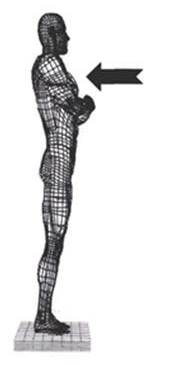
\includegraphics[width=0.22\linewidth]{human_3.png}
    \caption{Cхематическое изображение толкателя и
        положения испытуемого на стабилоплатформе}
    \label{fig:pusher}
\end{figure}

Исходные данные об отклонении сагиттальной коордианты при различных по силе толчках, предоставлены сотрудниками ИМБП РАН (см. рисунок \ref{fig:pushes})
\begin{figure}[h!]
    \centering
    \includegraphics[width=1\linewidth]{sagg_and_pushes.eps}
    \caption{Отклонение сагиттальной координаты при различных по силе толчках}
    \label{fig:pushes}
\end{figure}

В качестве математической модели
используется традиционно модель «перевернутого маятника»\cite{PAKrychinin,gurfincel}.


\textbf{Целью работы} является разработка алгоритма управления изменением позы человека, основанного на решении задачи оптимального быстродействия,
который можно было бы использовать для возвращения в исходную вертикальную позу. В дальнейшем
такое решение предполагается использовать для оценки эффективности управления человеком
при возвращении в вертикальную позу, путем сравнения
времени реального процесса с полученным эталонным решением оптимальной задачи.

\textbf{Акутальность работы} объясняется тем, что в ряде организаций прводятся подобные тесты, например в ИМБП РАН, но их анализ затруднен.
Одной из причин является сложность создания фиксированных условий толчка и его силы. Предлагаемая работа призвана преодолеть эту проблему.
Решение этой задачи может быть применено в медицине для оценки оптимальности работы мышщ человека, оценки качества выполнения заданного движения
при толчках заданной величины, например для космонавтов или спортсменов.

\textbf{Задачи работы: }
\begin{itemize}
    \item Описание математической модели
    \item Постановка задачи быстродействия, используя принцип максимума Понтрягина
    \item Поиск решения задачи быстродействия
    \item Определение начального состояния системы, в момент завершения толчка
    \item Решение задачи быстродействия с вычисленными начальными условиям
    \item Сравнение реального и оптимального времени возвращения в исходную позу
    \item Сравнение реальной и оптимальной траектории возвращения в исходную позу
    \item Интерпретация полученных результатов
\end{itemize}

\textbf{Методы исследования:}
\begin{itemize}
    \item Движение человека в саггитальной плоскости описывается моделью перевернутого маятника.
    \item Для описания движения используется система обыкновенных дифференциальных уравнений с постоянными коэффицентами 3 порядка.
    \item Начальные условия для задачи быстродействия определяются с данных эксперимента, в ходе которого на человека оказывают толкающее воздействие.
    \item Проводится математическое моделирование в пакетах Matlab R2022a и Wolfram Mathematica 13.0.
\end{itemize}




\textbf{Объем и структура работы.} Работа состоит из введения, трех глав и заключения. Полный объем работы составляет
32 страниц, включая 21 рисунок и 2 таблицы.

\newpage

\chapter{Математическая модель и решение задачи быстродействия}
\section{Математическая модель}
Для описания движения тела человека в сагиттальной плоскости используем традиционную модель перевернутого маятника (см. рисунок \ref{fig:pendulum}).

\begin{figure}[h!]
    \centering
    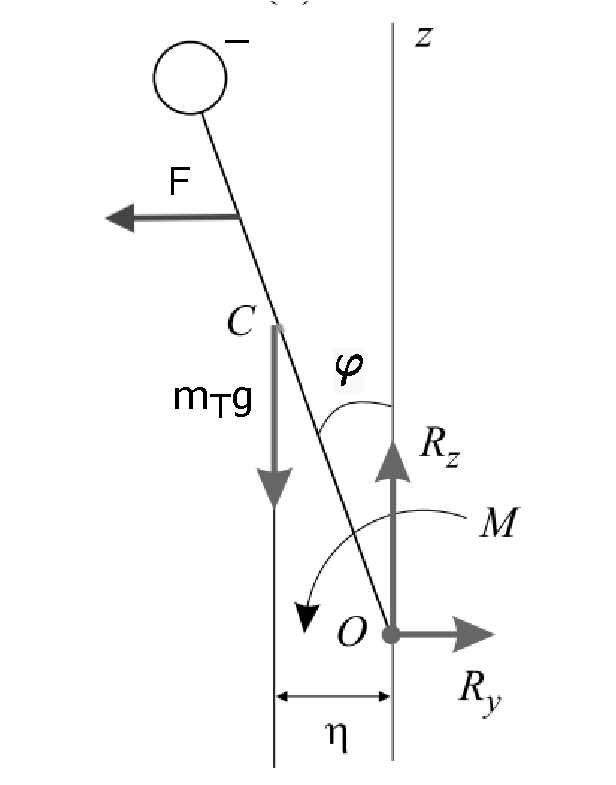
\includegraphics[width=0.4\linewidth]{body_1.pdf}
    \caption{Модель перевернутого маятника}
    \label{fig:pendulum}
\end{figure}

Традиционно предполагаем, что тело человека в ходе теста допустимо
моделировать недеформируемым однородным стержнем массы $m_T$,
закрепленным шарнирно в точке $O$, которая соответствует
голеностопному суставу.

Центр масс стержня расположен в точке $C$, удаленной от точки $O$
на расстояние $l$. Момент инерции стержня относительно фронтальной
оси, проходящей через точку $O$, равен $J$. Отклонение стержня от
вертикали описывается углом $\varphi$. Будем считать, что обследуемый
ориентирован так, что его сагиттальная плоскость параллельна оси
чувствительности платформы, а его стопа неподвижна относительно
платформы. Скорость изменения момента $M$, который приложен в точке $O$ к стержню,
будем считать управлением.

$R_z - $вертикальная реакция со стороны ступни,

$R_y - $горизонтальная реакция со стороны ступни,

$F - $ сила с которой толкают человека,

$g - $ускорение свободного падения,

$\eta - $ саггитальная координата центра масс.

На тело воздействует два момента: первый от силы тяжести, второй момент создают мышцы голеностопного сустава.
Запишем уравнение моментов,относительно точки $O$ на ось перпендикулярную плоскости рисунка \ref{fig:pendulum}
\[
    J\ddot{\varphi}= m_Tgl\sin\varphi+M
\]

Уравнение моментов для малых значений угла $\varphi$ и
скорости его изменения запишем, как традиционно принято для этой задачи.
\[
    J\ddot{\varphi}= m_Tgl\varphi+M
\]

Необходимо перевести решение уравнения из начального состояния,
где $\varphi_0-$  значение угла отклонения после толчка,
$\omega_0-$  значение угловой скорости после толчка
\[
    \varphi(0)=\varphi_0, \,\dot{\varphi}(0)=\omega_0
\]

в конечное состояние
\[
    \varphi(t_k)=\varphi_k,\, \dot{\varphi}(t_k)=0.
\]
$\varphi_k - $ конечное значение угла отклоенения тела, после стабилизации позы


При этом будем принимать во внимание
условия ограниченности величины момента в голеностопном суставе
\begin{equation}\label{moments_cond}
    M^-\leqslant M\leqslant\ M^+.
\end{equation}

$M^+ -$ максимальный развиваемый момент в голеностопном суставе

$M^- -$ минимальный развиваемый момент в голеностопном суставе

Для величины момента помимо чисто физиологических ограничений, связанных с ограниченностью развиваемых мышечных усилий, следует принимать во внимание возможность опрокидывания человека вследствие того, что
равновесие стоп на платформе должно обеспечиваться нормальной реакцией, приложенной в области опоры.
В нашей постановке задачи, человек не опрокидывается после толчков и точка приложения нормальной реакции опоры не выходит за пределы стопы, поэтому пренебрежем \eqref{moments_cond}

Будем принимать во внимание условия ограниченности скорости изменения
момента в голеностопном суставе, как это соответствует физиологически
\[
    U^-\leqslant\dot{M}\leqslant\ U^+.
\]

$U^+ -$ максимальная развиваемая скорость изменения момента в голеностопном суставе

$U^- -$ минимальная развиваемая скорость изменения момента в голеностопном суставе

Перевод состояния тела должен происходить за минимальное
время $t_k$, с помощью изменений значения $\dot{M}$ в
голеностопном суставе.

Будем считать, что за время толчка система регуляции позы человека
не успела среагировать и момент в голеностопном суставе остался
неизменным и соответствует значению, обеспечивающему положение
равновесия человека до начала движения и после его завершения
\[
    M(0)=M\left(t_k\right)=-m_Tgl\varphi_k;
\]
Для дальнейшего анализа задачи представим приведенные
соотношения в безразмерном виде. Для этого перейдем
к новым переменным
\[
    \theta=\frac{\varphi-\varphi_k}{\varphi_\ast},\ \ m=\frac{M-M_f}{m_Tgl\varphi_\ast}.
\]

В качестве характерного значения угла выберем разность
начального и конечного значений угла в голеностопном
суставе при выполнении пробы $\varphi_\ast=\varphi_0-\varphi_k$

Введем безразмерное время
\[
    \tau=\frac{t}{t_\ast},\ t_\ast=\sqrt{\frac{J}{m_Tgl}}.
\]

Управлением $u$ будем считать скорость изменения безразмерного
момента. Для этих переменных обезразмеренные уравнения движения
примут следующий вид
\begin{equation}\label{system}
    \theta^{''}=\theta+m;\ m^{'}=u
\end{equation}

Здесь через $m^{'}$ обозначено дифференцирование по
безразмерному времени $\tau$. Тогда необходимо решение системы \eqref{system}
перевести из начального положения
\[
    \theta(0)=1;\ \theta^{'}(0)=\frac{t_\ast}{\varphi_\ast}\omega_0=\Omega_0;\ m(0)=0
\]
в положение
\[
    \theta(\tau_f)=0;\ \theta^{'}(\tau_f)=0;\ m(\tau_f)=0
\]
с помощью ограниченного управления
\[
    u^-\leqslant\ u\leqslant\ u^+,\ \text{где}
\]
\[
    u^-=\frac{t_\ast U^-}{m_Tgl\varphi_\ast },\ \ u^+=\frac{t_\ast U^+}{m_Tgl\varphi_\ast}.
\]
Далее будем считать, что $|u^-|=|-u^+|=u_\ast=u_{max}$

\section{Постановка задачи быстродействия}

Выпишем систему \eqref{system} в форме Коши
\begin{equation}\label{koshisystem}
    \left\{ {\begin{aligned}
                 & \theta^{'} = \omega , \hfill   \\
                 & \omega^{'} = \theta+m , \hfill \\
                 & m^{'} = u . \hfill             \\
            \end{aligned}} \right.
\end{equation}

Ограничение на управление $|u|\leqslant u_{max}$

Начальные условия
\[
    \theta(0)=1;\ \omega(0)=\frac{t_\ast}{\varphi_\ast}\omega_0=\Omega_0;\ m(0)=0
\]

Конечные условия
\[
    \theta(\tau_f)=0;\ \theta^{'}(\tau_f)=0;\ m(\tau_f)=0
\]


Для решения задачи оптимального быстродействия $J=\tau_f\to \min$ будем использовать принцип максимума Понтрягина \cite{Optimal}:

Если $\{y^0(\cdot),u^0(\cdot),[t_0,t_k^0]\} - $ оптимальный процесс, то существует нетривиальная пара $\{\lambda_0\geq0,\psi(\cdot)\}$
такая, что
\begin{itemize}
    \item $ \mathop {\max }\limits_{u(t) \in \Omega}  H(\psi(t),y^0(t),u(t))=H(\psi(t),y^0(t),u^0(t))$
          $\forall t \in T \subseteq [t_0,t_k^0];$
    \item $\psi(t_k^0)+\lambda_0(\frac{\partial \varphi_0(y^0(t_k^0))}{\partial y})^T \perp M \text{ в точке } y^0(t_k^0);$
    \item $\mathcal{H}=H(\psi(t),y^0(t),u^0(t))\equiv0 \text{ при } t \in [t_0,t_k^0].$
\end{itemize}
Запишем функцию Понтрягина
\[
    H(\psi(t),y(t),u(t))=\psi_1\cdot\omega+\psi_2\cdot(\theta+m)+\psi_3\cdot u
\]
Сопряженная система уравнений:
\[
    \psi^{'}_i  =  - \frac{{\partial H}}{{\partial y_i }},\,\,i = 1, \ldots ,n
\]
В данной задаче $y_1 = \theta, y_2 = \omega, y_3=m$, тогда сопряженная система примет вид
\begin{equation} \label{7}
    \left\{ {\begin{aligned}
                 & \psi^{'}_1=  - \frac{{\partial H}}{{\partial \theta}} = - \psi_2\hfill  \\
                 & \psi^{'}_2=  - \frac{{\partial H}}{{\partial \omega }} = - \psi_1\hfill \\
                 & \psi^{'}_3=  - \frac{{\partial H}}{{\partial m }} = - \psi_2 \hfill     \\
            \end{aligned}} \right.
\end{equation}

\section{Анализ задачи быстродействия}
Проверим управляемость системы \eqref{koshisystem}.

(Критерий управляемости Калмана) Линейная стационарная система (11) вполне управляема на отрезке [0, T] тогда и
только тогда, когда матрица $W = \{B, AB, A^2B, ..., A^{n-1}B\}$ имеет ранг, равный n.

Для системы \eqref{koshisystem} матрицы $A, B, W$ равны соответственно
$$ A =
    \begin{pmatrix}
        0 & 1 & 0 \\
        1 & 0 & 1 \\
        0 & 0 & 0
    \end{pmatrix};
    \quad
    B =
    \begin{pmatrix}
        0 \\
        0 \\
        1
    \end{pmatrix};
    \quad
    W =
    \begin{pmatrix}
        0 & 0 & 1 \\
        0 & 1 & 0 \\
        1 & 0 & 0
        \end{pmatrix}
$$
$rank (W)=3$, значит система полностью управляема

Рассмотрим собственные числа системы \eqref{koshisystem}
\begin{equation}\label{eugen_values}
    \det \left( {{\mathcal{A}} - \lambda\,\mathcal{I}} \right) = 0 \Longleftrightarrow \begin{vmatrix}
        -\lambda & 1        & 0        \\
        1        & -\lambda & 1        \\
        0        & 0        & -\lambda
    \end{vmatrix} = 0,
\end{equation}
где $\mathcal{I}$ -- единичная матрица.

Раскрывая определитель, получим $\lambda_1=0, \quad \lambda_2=1,\quad \lambda_3=-1$,
в литературе \cite{atansfalb} нет готового решения, для задач с нулевыми собственными значениями.

При $\psi_3\equiv0$ следует, что $\psi_2\equiv0$ и $\psi_1\equiv0$ следовательно особого управления нет.

Тогда для условия максимизации функции Понтрягина
\[
    u=
    \begin{cases}
        -u_{max}, & \text{при $\psi_3<0$}          \\
        +u_{max}, & \text{при $\psi_3\geqslant 0$}
    \end{cases}
\]\\*
Продифференцируем по безразмерному времени второе уравнение из \eqref{7} и подставим в него первое, получим
\[
    \psi_2 ''=\psi_2
\]
Решая систему \eqref{7}, получим
\[
    \left\{ {\begin{aligned}
                 & \psi_1 = -C_1e^\tau+C_2e^{-\tau}+C_3, \hfill  \\
                 & \psi_2 = C_1e^\tau+C_2e^{-\tau} , \hfill      \\
                 & \psi_3 = -C_1e^\tau+C_2e^{-\tau}+C_3 . \hfill \\
            \end{aligned}} \right.
\]

Анализируя корни уравнения $\psi_3(\tau)=0$, для различной комбинации
коэффициентов $C_1,C_2,C_3$, получим, что число корней не может быть больше двух. В системе может быть не более двух переключений $u$.

Аналагичный вывод можно получить, применив к решаемой задаче теорему Фельдбаума о числе переключений оптимального управления\cite{feldbaum}



\section{Решение задачи быстродействия на отдельных этапах времени}
Выбор знака + или - перед определяется на основании полученных корней,
одно из решений явно будет не подходящим, исходя из физической реализации процесса.

Для определенности возьмем $u=-u_\ast$, управление на первом участке траектории до первого переключения.

Пусть первое переключение управления происходит в момент времени
$\tau=\tau_1$, а второе в момент времени
$\tau=\tau_2$. Рассмотрим систему \eqref{koshisystem} на трех этапах,
при переходе между которыми меняется управление.

Решая систему \eqref{koshisystem}, получим

\begin{equation}\label{solvekoshi}
    \left\{ {\begin{aligned}
                 & m(\tau) = \tau u+C_1, \hfill                                                            \\
                 & \theta(\tau) = \frac{1}{2} e^{-\tau } \left((C_1+C_2+C_3) e^{2 \tau }-2 e^{\tau } (\tau
                u+C_1)+C_1+C_2-C_3\right), \hfill                                                          \\
                 & \omega(\tau) = \frac{1}{2} e^{-\tau } \left((C_1+C_2+C_3) e^{2 \tau }-2 e^{\tau }
                u-C_1-C_2+C_3\right). \hfill                                                               \\
            \end{aligned}} \right.
\end{equation}

\subsection*{Решение системы на первом этапе}
Этап 1. $u=-u_*$ начальные условия
\[
    m(0)=0;\ \theta(0)=1;\ \omega(0)=\Omega_0;
\]

Из \eqref{solvekoshi} получим
\[
    \left\{ {\begin{aligned}
                 & 0 = -\tau  u_*+c_1, \hfill                                                            \\
                 & 1 = \frac{1}{2} e^{-\tau } \left(C_1 \left(e^{\tau }-1\right)^2+C_2 \left(e^{2
                \tau }+1\right)+C_3 e^{2 \tau }-C_3+2 e^{\tau } \tau  u_*\right) , \hfill                \\
                 & \Omega_0 = \frac{1}{2} e^{-\tau } \left(C_1 \left(e^{2 \tau }-1\right)+C_2 \left(e^{2
                \tau }-1\right)+C_3 e^{2 \tau }+C_3+2 e^{\tau } u_*\right)  . \hfill                     \\
            \end{aligned}} \right.
\]
Тогда
\[
    \left\{ {\begin{aligned}
                 & C_1 = 0, \hfill             \\
                 & C_2 = 1, \hfill             \\
                 & C_3 = -u_*+\Omega_0. \hfill \\
            \end{aligned}} \right.
\]
Подставим полученные константы в \eqref{solvekoshi}
\[
    \left\{ {\begin{aligned}
                 & m_1(\tau) = -\tau  u_*, \hfill                                                                         \\
                 & \theta_1(\tau) = \frac{e^\tau+e^{-\tau}}{2}+\frac{\Omega_0-u_*}{2}(e^\tau-e^{-\tau})+\tau u_* , \hfill \\
                 & \omega_1(\tau) =\frac{e^\tau-e^{-\tau}}{2}+\frac{\Omega_0-u_*}{2}(e^\tau+e^{-\tau})+u_*   . \hfill     \\
            \end{aligned}} \right.
\]
\subsection*{Решение системы на втором этапе}
Этап 2. $u=u_*$ начальные условия
\[
    m(\tau_1)=m_1(\tau_1); \ \theta(\tau_1)=\theta_1(\tau_1);\ \omega(\tau_1)=\omega_1(\tau_1);
\]
\[
    \left\{ {\begin{aligned}
                 & m(\tau_1) = -\tau _1 u_*, \hfill                                                            \\
                 & \theta(\tau_1) = \frac{1}{2} e^{-\tau _1} \left(\left(e^{2 \tau _1}-1\right) \Omega _0+e^{2
                \tau _1}+\left(2 e^{\tau _1} \tau _1-e^{2 \tau _1}+1\right) u_*+1\right) , \hfill              \\
                 & \omega(\tau_1) = \frac{1}{2} e^{-\tau _1} \left(\left(e^{2 \tau _1}+1\right) \Omega
                _0-\left(e^{\tau _1}-1\right) \left(-e^{\tau _1}+\left(e^{\tau
                _1}-1\right) u_*-1\right)\right) . \hfill                                                      \\
            \end{aligned}} \right.
\]
Находим константы интегрирования
\[
    \left\{ {\begin{aligned}
                 & -\tau _1 u_* = \tau _1 u_*+C_1, \hfill                                         \\
                 & \frac{1}{2} e^{-\tau _1} \left(\left(e^{2 \tau _1}-1\right) \Omega _0+e^{2
                \tau _1}+\left(2 e^{\tau _1} \tau _1-e^{2 \tau _1}+1\right) u_*+1\right) =        \\
                 & = \frac{1}{2} e^{-\tau _1} \left(C_1 \left(e^{\tau _1}-1\right){}^2+C_2 e^{2
                \tau _1}+C_3 e^{2 \tau _1}-2 e^{\tau _1} \tau _1 u_*+C_2-C_3\right) , \hfill      \\
                 & \frac{1}{2} e^{-\tau _1} \left(\left(e^{2 \tau _1}+1\right) \Omega
                _0-\left(e^{\tau _1}-1\right) \left(-e^{\tau _1}+\left(e^{\tau
                _1}-1\right) u_*-1\right)\right)=                                                 \\
                 & =\frac{1}{2} e^{-\tau _1} \left(C_1 \left(e^{2 \tau _1}-1\right)+C_2 e^{2 \tau
                _1}+C_3 e^{2 \tau _1}-2 e^{\tau _1} u_*-C_2+C_3\right)  . \hfill                  \\
            \end{aligned}} \right.
\]
\[
    \left\{ {\begin{aligned}
                 & C_1 =-2 \tau _1 u_*, \hfill                                                    \\
                 & C_2 = -e^{-\tau _1} \left(-e^{\tau _1}+e^{2 \tau _1} u_*-2 e^{\tau _1} \tau _1
                u_*-u_*\right), \hfill                                                            \\
                 & C_3 = e^{-\tau _1} \left(e^{\tau _1} \Omega _0-e^{\tau _1} u_*+e^{2 \tau _1}
                u_*+u_*\right). \hfill                                                            \\
            \end{aligned}} \right.
\]

Подставим начальные условия для второго этапа в \eqref{solvekoshi}, получим

\[
    \left\{ {\begin{aligned}
                 & m_2(\tau) = \left(\tau -2 \tau _1\right) u_*, \hfill                                                                                                \\
                 & \theta_2(\tau) = \frac{e^\tau+e^{-\tau}}{2}+\frac{\Omega_0-u_\ast}{2}(e^\tau-e^{-\tau})+u_*(e^{\tau-\tau_1}-e^{-\tau+\tau_1}+2\tau_1-\tau) , \hfill \\
                 & \omega_2(\tau) = \frac{e^\tau-e^{-\tau}}{2}+\frac{\Omega_0-u_\ast}{2}(e^\tau+e^{-\tau})+u_*(e^{\tau-\tau_1}+e^{-\tau+\tau_1}-1) . \hfill            \\
            \end{aligned}} \right.
\]
\subsection*{Решение системы на третьем этапе}
Этап 3. $u=-u_*$ конечные условия
\[
    m(\tau_f)=0; \ \theta(\tau_f)=0;\ \omega(\tau_f)=0;
\]
Подставим начальные условия в \eqref{solvekoshi}, получим
\[
    \left\{ {\begin{aligned}
                 & 0 = C_1-\tau_f  u_*, \hfill                                               \\
                 & 0 = \frac{1}{2} e^{-\tau _f} \left(C_1 \left(e^{\tau _f}-1\right){}^2+C_2
                \left(e^{2 \tau _f}+1\right)+C_3 e^{2 \tau _f}-C_3+2 u_* e^{\tau _f} \tau
                _f\right), \hfill                                                            \\
                 & 0 = \frac{1}{2} e^{-\tau _f} \left(C_1 \left(e^{2 \tau _f}-1\right)+C_2
                \left(e^{2 \tau _f}-1\right)+C_3 e^{2 \tau _f}+C_3+2 u_* e^{\tau
                _f}\right)  . \hfill                                                         \\
            \end{aligned}} \right.
\]
\[
    \left\{ {\begin{aligned}
                 & C_1 = u_* \tau _f, \hfill                                                  \\
                 & C_1 = \frac{1}{2} u_* e^{-\tau _f} \left(-2 e^{\tau _f} \tau _f+e^{2 \tau
                _f}-1\right), \hfill                                                          \\
                 & C_2 = -\frac{1}{2} u_* e^{-\tau _f} \left(e^{2 \tau _f}+1\right)  . \hfill \\
            \end{aligned}} \right.
\]
Тогда решение на этом этапе имеет вид
\[
    \left\{ {\begin{aligned}
                 & m_3(\tau) = u_* \left(\tau _f-\tau \right), \hfill                                           \\
                 & \theta_3(\tau) = \frac{1}{2} u_* \left(-e^{\tau -\tau _f}+e^{\tau _f-\tau }-2 \tau _f+2 \tau
                \right), \hfill                                                                                 \\
                 & \omega_3(\tau) =u_*-\frac{u_*}{2}(e^{\tau-\tau_f}+e^{-\tau+\tau_f}) . \hfill                 \\
            \end{aligned}} \right.
\]

\subsection*{Сопряжение второго и третьего этапов}

Так как момент, угол отклонения и угловая скорость представлют собой кусочно-непрерывные фукнции времени,
то можно сопрячь систему на втором и третьем этапе в момент времени $\tau_2$.
\[
    \left\{ {\begin{aligned}
                 & m_2(\tau_2) = m_3(\tau_2), \hfill            \\
                 & \theta_2(\tau_2) =  \theta_3(\tau_2), \hfill \\
                 & \omega_2(\tau_2) = \omega_3(\tau_2) . \hfill \\
            \end{aligned}} \right.
\]
Получим
\[
    \left\{
    \begin{multlined}
        \left(\tau _2-2 \tau _1\right) u_*=u_* \left(\tau _f-\tau _2\right), \\
        % 2-nd equation
        \shoveleft{\frac{e^{\tau_2}+e^{-\tau_2}}{2}+\frac{\Omega_0-u_\ast}{2}(e^{\tau_2}-e^{-\tau_2})+u_*(e^{\tau_2-\tau_1}-e^{-\tau_2+\tau_1}+2\tau_1-\tau_2)=} \\
        \shoveleft{=\frac{1}{2} u_* \left(-e^{\tau _2-\tau _f}+e^{\tau _f-\tau _2}-2 \tau _f+2
            \tau _2\right),} \\
        % 4-th equation
        \shoveleft{\frac{e^{\tau_2}-e^{-\tau_2}}{2}+\frac{\Omega_0-u_\ast}{2}(e^{\tau_2}+e^{-\tau_2})+u_*(e^{\tau_2-\tau_1}+e^{-\tau_2+\tau_1}-1)=} \\
        \shoveleft{=u_*-\frac{u_*}{2}(e^{\tau_2-\tau_f}+e^{-\tau_2+\tau_f}).} \\
    \end{multlined}
    \right.
\]

Сократим первое уравнение на $u_*$, выражение для $\tau_f$ из первого уравнения подставим во второе и третье
\begin{equation}\label{fullconnected}
    \left\{ {\begin{aligned}
                 & \tau_f=2(\tau_2-\tau_1),                                                                                                                                                                 \\
                 & \frac{e^{\tau_2}+e^{-\tau_2}}{2}+\frac{\Omega_0-u_*}{2}(e^{\tau_2}-e^{-\tau_2})+u_*\left(e^{-\tau_1+\tau_2}-e^{\tau_1-\tau_2}+\frac{e^{\tau_2-\tau_f}-e^{-\tau_2+\tau_f}}{2}\right)=0,   \\
                 & \frac{e^{\tau_2}-e^{-\tau_2}}{2}+\frac{\Omega_0-u_*}{2}(e^{\tau_2}+e^{-\tau_2})+u_*\left(e^{\tau_1-\tau_2}+e^{-\tau_1+\tau_2}+\frac{e^{\tau_2-\tau_f}+e^{-\tau_2+\tau_f}}{2}-2\right)=0. \\
            \end{aligned}} \right.
\end{equation}

Введем замену переменных
\[
    x=e^{\tau_1} ,\,\,y=e^{\tau_2} ,\,\,z=e^{\frac{\tau_f}{2}}
\]
\[
    \left\{ {\begin{aligned}
                 & z=\frac{y}{x}, \hfill                                                         \\
                 & \frac{1}{2} \left(u_* \left(\frac{x^2}{y}-\frac{y}{x^2}-\frac{2 x}{y}+\frac{2
                        y}{x}-y+\frac{1}{y}\right)+\left(y-\frac{1}{y}\right) \Omega
                _0+y+\frac{1}{y}\right)=0, \hfill                                                \\
                 & \frac{u_* \left(\frac{y^2}{x^2}+x^2+\frac{2 y^2}{x}+2 x-y^2-4
                y-1\right)+\left(y^2+1\right) \Omega _0+y^2-1}{2 y}=0. \hfill                    \\
            \end{aligned}} \right.
\]
\begin{equation}\label{fullchanged}
    \left\{ {\begin{aligned}
                 & z=\frac{y}{x}, \hfill                                                                                                              \\
                 & (\Omega_0-u_*)\left( xy-\frac{x}{y}\right)+u_*\left(\frac{x^3}{y}-\frac{y}{x}-\frac{2x^2}{y}+2y\right)+\frac{x}{y}+xy=0, \hfill    \\
                 & (\Omega_0-u_*)\left( xy+\frac{x}{y}\right)+u_*\left(\frac{x^3}{y}+\frac{y}{x}+\frac{2x^2}{y}+2y-4x\right)-\frac{x}{y}+xy=0. \hfill \\
            \end{aligned}} \right.
\end{equation}

Полученную систему \eqref{fullchanged} можно решить численно, подставив вместо $\Omega_0$ и $u_\ast$ конкретные значения.
Отбор корней проводим из условия, что $x>1,y>1,z>1$.
Но также стоит провести дальнейший анализ для поиска аналитического решения.
\section{Сведение задачи к отысканию корней полинома}

\begin{equation}\label{fullchanged1}
    \left\{ {\begin{aligned}
                 & y=zx, \hfill                                                                                                                                 \\
                 & (\Omega_0-u_*)\left( x^2z-\frac{x}{zx}\right)+u_*\left(\frac{x^3}{zx}-\frac{zx}{x}-\frac{2x^2}{zx}+2zx\right)+\frac{x}{zx}+x^2z=0, \hfill    \\
                 & (\Omega_0-u_*)\left( x^2z+\frac{x}{zx}\right)+u_*\left(\frac{x^3}{zx}+\frac{zx}{x}+\frac{2x^2}{zx}+2zx-4x\right)-\frac{x}{zx}+x^2z=0. \hfill \\
            \end{aligned}} \right.
\end{equation}
\begin{equation}
    \left\{ {\begin{aligned}
                 & (\Omega_0-u_*)\left( x^2z-\frac{1}{z}\right)+u_*\left(\frac{x^2}{z}-z-\frac{2x}{z}+2zx\right)+\frac{1}{z}+x^2z=0, \hfill    \\
                 & (\Omega_0-u_*)\left( x^2z+\frac{1}{z}\right)+u_*\left(\frac{x^2}{z}+z+\frac{2x}{z}+2zx-4x\right)-\frac{1}{z}+x^2z=0. \hfill \\
            \end{aligned}} \right.
\end{equation}
Сложим и вычтем уравнения системы
\begin{equation}
    \left\{ {\begin{aligned}
                 & 2(\Omega_0-u_*)x^2z+u_*\left(2\frac{x^2}{z}+4zx-4x\right)+2x^2z=0, \hfill           \\
                 & 2(\Omega_0-u_*)\frac{1}{z}+u_*\left(2z+\frac{4x}{z}-4x\right)-\frac{2}{z}=0. \hfill \\
            \end{aligned}} \right.
\end{equation}
\begin{equation}
    \left\{ {\begin{aligned}
                 & 2(\Omega_0-u_*)x^2z+u_*\left(2\frac{x^2}{z}+4zx-4x\right)+2x^2z=0, \hfill               \\
                 & 2(\Omega_0-u_*)\frac{1}{z}+2u_*z+4x\left(\frac{u_*}{z}-u_*\right)-\frac{2}{z}=0. \hfill \\
            \end{aligned}} \right.
\end{equation}
\begin{equation}
    \left\{ {\begin{aligned}
                 & 2(\Omega_0-u_*)x^2z+u_*\left(2\frac{x^2}{z}+4zx-4x\right)+2x^2z=0, \hfill                       \\
                 & x=\left( \frac{1}{2z}-\frac{u_*z}{2}-(\Omega_0-u_*)\frac{1}{2z}\right)\frac{z}{u_*(1-z)} \hfill \\
            \end{aligned}} \right.
\end{equation}
\[
    \frac{\left(u_* \left(z^2-1\right)+\Omega _0-1\right) \left(-u_* \left(z^4+\Omega _0 \left(z^2-1\right)^2\right)+u_*^2 (z-1)^4+u_*-\Omega _0^2 z^2+z^2\right)}{2 u_*^2 (z-1)^2}=0
\]
\begin{equation}
    \left[ {\begin{aligned}
                 & \left(u_* \left(z^2-1\right)+\Omega _0-1\right)=0, \hfill                                           \\
                 & -u_* \left(z^4+\Omega _0 \left(z^2-1\right)^2\right)+u_*^2 (z-1)^4+u_*-\Omega _0^2 z^2+z^2=0 \hfill \\
            \end{aligned}} \right.
\end{equation}
\begin{equation}\label{final_polynom}
    \left[ {\begin{aligned}
                 & u_*z^2+\Omega _0-1-u_*=0, \hfill                                                                                               \\
                 & (-u_* \Omega _0+u_*^2-u_*)z^4-4 u_*^2z^3+(2 u_* \Omega _0+6 u_*^2-\Omega _0^2+1)z^2-4 u_*^2z+-u_* \Omega _0+u_*^2+u_*=0 \hfill \\
            \end{aligned}} \right.
\end{equation}

Дальнейшее решение строится на основе перебора знака $u_\ast$, выбор знака + или - определяется на основании полученных корней,
одно из решений явно будет не подходящим, исходя из физической реализации процесса.
\section{Решение задачи быстродействия при $n<2$ переключений управления}
Пусть в системе \eqref{koshisystem} \textbf{нет переключений управления}, тогда 
\[
    m(\tau) = \tau u, 
\]
$m(\tau_f)=0$, тогда либо $u\equiv0$, либо $\tau=0$, чего не может быть, так как тогда решение \eqref{koshisystem} будет неограниченно возрастать

Пусть в системе \eqref{koshisystem} \textbf{одно переключение управления}, тогда пусть переключение идет в момент времени $\tau_1$.

Этап 1. $u=-u_*$ начальные условия
\[
    m(0)=0;\ \theta(0)=1;\ \omega(0)=\Omega_0;
\]
\begin{equation}\label{solvekoshi}
    \left\{ {\begin{aligned}
                 & m_1(\tau) = u_* \tau, \hfill                                                            \\
                 & \theta_1(\tau) = \frac{1}{2} e^{\tau } \left(-u_*+\Omega _0+1\right)+\frac{1}{2} e^{-\tau } \left(u_*-\Omega _0+1\right)+\tau  u_*, \hfill                                                          \\
                 & \omega_1(\tau) = \frac{1}{2} e^{-\tau } \left(-u_*+\Omega _0-1\right)+\frac{1}{2} e^{\tau } \left(-u_*+\Omega _0+1\right)+u_*. \hfill                                                               \\
            \end{aligned}} \right.
\end{equation}

Этап 2. $u=u_*$ конечные условия
\[
    m(\tau_f)=0; \ \theta(\tau_f)=0;\ \omega(\tau_f)=0;
\]
\begin{equation}\label{solvekoshi}
    \left\{ {\begin{aligned}
                 & m_2(\tau) = u_* \left(\tau-\tau _f\right), \hfill                                                            \\
                 & \theta_2(\tau) = \frac{1}{2} u_* e^{\tau -\tau _f}-\frac{1}{2} u_* e^{\tau _f-\tau }+\frac{1}{2} u_* \left(2 \tau _f-2 \tau \right), \hfill                                                          \\
                 & \omega_2(\tau) = \frac{1}{2} u_* e^{\tau -\tau _f}+\frac{1}{2} u_* e^{\tau _f-\tau }-u_*. \hfill                                                               \\
            \end{aligned}} \right.
\end{equation}

Сопряжем 1 и 2 этапы из условия
\[
    \left\{ {\begin{aligned}
                 & m_1(\tau_1) = m_2(\tau_1), \hfill            \\
                 & \theta_1(\tau_1) =  \theta_2(\tau_1), \hfill \\
                 & \omega_1(\tau_1) = \omega_2(\tau_1) . \hfill \\
            \end{aligned}} \right.
\]
Получим
\[
    \left\{ {\begin{aligned}
                 & 2 \tau _1 u_*=u_* \tau _f, \hfill            \\
                 & -u_* e^{\tau _1-\tau _f}+u_* e^{\tau _f-\tau _1}-2 u_* \tau _f-e^{-\tau _1} \Omega _0+e^{\tau _1} \Omega _0+e^{-\tau _1}+e^{\tau _1}+e^{-\tau _1} u_*-e^{\tau _1} u_*+4 \tau _1 u_*=0, \hfill \\
                 & u_* e^{\tau _1-\tau _f}+u_* e^{\tau _f-\tau _1}-e^{-\tau _1} \Omega _0-e^{\tau _1} \Omega _0+e^{-\tau _1}-e^{\tau _1}+e^{-\tau _1} u_*+e^{\tau _1} u_*-4 u_*=0. \hfill \\
            \end{aligned}} \right.
\]
Подставим первое уравнение $\tau_f=2\tau_1$ во второе и третье
\begin{equation}\label{1_control_syst}
    \left\{ {\begin{aligned}
                 & 2 \tau _1=\tau _f, \hfill            \\
                 & e^{-\tau _1} \left(1-\Omega _0\right)+e^{\tau _1} \left(\Omega _0+1\right)=0, \hfill \\
                 & e^{\tau _1} \left(2 u_*-\Omega _0-1\right)+e^{-\tau _1} \left(2 u_*-\Omega _0+1\right)-4 u_*=0. \hfill \\
            \end{aligned}} \right.
\end{equation}
            
Сделаем замену $e^{\tau_1}=x;\quad e^{\tau_f}=z$

Тогда \eqref{1_control_syst} примет вид
\begin{equation}\label{1_control_syst_subst}
    \left\{ {\begin{aligned}
                 & x^2 = z, \hfill            \\
                 & \dfrac{1}{x}(1-\Omega_0)+x(1+\Omega_0)=0, \hfill \\
                 & x \left(2 u_*-\Omega _0-1\right)+\dfrac{1}{x}\left(2 u_*-\Omega _0+1\right)-4 u_*=0. \hfill \\
            \end{aligned}} \right.
\end{equation}

Из второго уравнения \eqref{1_control_syst_subst} получим
$$x^2=\dfrac{\Omega_0-1}{\Omega_0+1}=1-\dfrac{2}{1+\Omega_0}$$

Будем считать, что толчок достаточно сильный, чтобы в момент завершения
 толчка начальная скорость была положительной, даже если мышцы уже
  будут оказывать некоторое сопротивление движению.

Используем предположение, что к концу толчка угол наклона продолжает увеличиваться и $\Omega_0>0$,
тогда $x<1$, чего не может быть.

\chapter{Определение начальных условий в момент завершения толчка}
\section{Постановка задачи}
Для корректного решения задачи быстродействия необходимо как можно лучше оценить
начальные условия в момент завершения толчка. Экспериментальные данные содержат только записи силомера
и стабилоанализатора, поэтому определять начальные условия будем на основе данных с саггитальной стабилограммы и силомера.

Рассмотрим силы действующие на модель стержня, иммитирующего тело человека (см. рисунок \ref{fig:pendulum})
и силы действующие на систему «стопы ног – платформа стабилоанализатора».
\begin{figure}[h!]
    \centering
    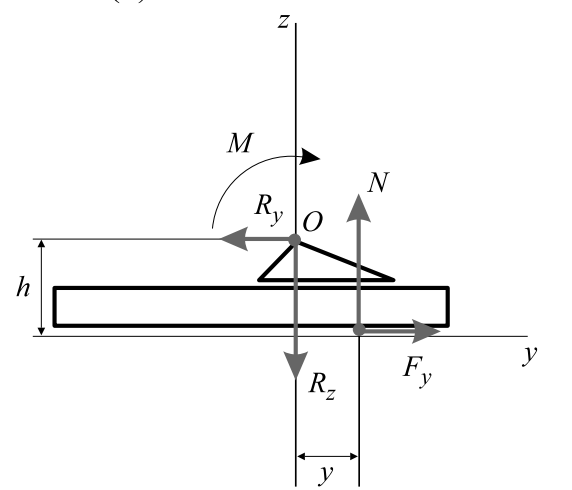
\includegraphics[width=0.5\linewidth]{foot.png}
    \caption{Силы действующие на на систему «стопы ног – платформа стабилоанализатора» }
    \label{fig:foot-platform}
\end{figure}

$F$ – это внешняя толкающая сила, $y$ – саггитальная координата центра давления, $l_1$ – высота точки к которой прикладывается толкающая сила
, $h$ – суммарная высота стопы и платформы стабилоанализатора, $N$ – вертикальная реакция опоры, $F_y$ – горизонтальная реакция опоры

Ниже представлена система уравнений соответствующая рисунку \ref{fig:pendulum}
\begin{equation}\label{bodyforces}
    \left\{ {\begin{aligned}
                 & m_Tl\ddot{\varphi} = -R_y-F , \hfill                             \\
                 & 0=R_z-m_Tg, \hfill                                              \\
                 & J \ddot{\varphi} = m_Tgl\sin \varphi-Fl_1\cos \varphi+M_x . \hfill \\
            \end{aligned}} \right.
\end{equation}
Проведем линеаризацию по $\varphi$ в окрестности нуля
\begin{equation}\label{bodyforces}
    \left\{ {\begin{aligned}
                 & m_Tl\ddot{\varphi} = -R_y-F , \hfill             \\
                 & 0=R_z-m_Tg, \hfill                              \\
                 & J \ddot{\varphi} = m_Tgl\varphi-Fl_1+M_x . \hfill \\
            \end{aligned}} \right.
\end{equation}
Ниже представлена система уравнений соответствующая рисунку \ref{fig:foot-platform}
\begin{equation}\label{footforces}
    \left\{ {\begin{aligned}
                 & M_x = Ny+F_yh , \hfill \\
                 & F_y = R_y , \hfill     \\
                 & N \approx m_Tg . \hfill  \\
            \end{aligned}} \right.
\end{equation}
Из \eqref{bodyforces} и \eqref{footforces} выразим $M_x$
$$M_x=m_Tgy-h\left(F+m_Tl\ddot{\varphi}\right)$$
Подставим $M_x$ в последнее уравнение системы \eqref{bodyforces} и сгруппируем слагемые с $\ddot{\varphi}$
$$\left(J+m_Tlh\right)\ddot{\varphi}=m_Tgl\varphi+m_Tgy-Fl_1-Fh$$
Разделим на $m_Tgl$
\begin{equation}\label{before_subst}
    \frac{(J+m_Tlh)l\ddot{\varphi}}{m_Tgl}=l\varphi+y-\frac{F}{m_Tg}(l_1+h);\quad
\end{equation}
Введем замену
$$\eta=-l\varphi; \quad T^2=\frac{J+m_Tlh}{m_Tgl};$$
Подставим замену в \eqref{before_subst}
\[
    T^2\ddot{\eta}=\eta-y+\frac{F}{m_Tg}(l_1+h)
\]

\begin{equation}\label{eta_y}
    T^2\ddot{\eta}=\eta-(y-\frac{F}{m_Tg}(l_1+h))
\end{equation}
Выражение \eqref{eta_y} можно свести к уравнению фильтра, путем корректировки входных данных $y$
\begin{equation}\label{eta_y_clear}
    T^2\ddot{\eta}=\eta-y
\end{equation}
Где $y -$  входные данные стабилоанализатора, $\eta -$ выходные данные оценки координаты центра масс

В работе \cite{kruchPodoprihin} получено такое же уравнение для связи центра масс и центра давления. Показано, что его решение неустойчиво и приводит к катастрофическому нарастанию ошибки оценки на временах больше 0.5c.

Для использования предположения об отсутствии экспоненциальных составляющих, порожденных решением однородного уравнения, запишем передаточную функцию, соответствующую
уравнению \eqref{eta_y_clear}
\begin{equation}\label{transf_func}
    G(s)=-\dfrac{1}{T^2s^2-1}
\end{equation}

В работе \cite{kruchPodoprihin} приведены два способа фильтрации данных: через преобразование Фурье и через фильрацию в прямом и обратном времени. Кратко опишем их.

\textbf{Фильтрация с использованием Фурье преобразования}: Рассмотрим Фурье-образы $N(\omega)$ и $Y(\omega)$ функций $\eta(t)$ и $y(t)$. В силу уравнения \eqref{transf_func} эти функции
связаны между собой соотношением.
\begin{equation}\label{transf_func_fur}
    N(\omega) = G(i\omega)Y(\omega).
\end{equation}
Представим функцию y(t) в виде суммы 
\begin{equation}\label{yt}
    y(t) = a(t - t_0) + b + \delta(t),
\end{equation}
где
\begin{equation}\label{ab}
    a=\dfrac{y(t_f)-y(t_0)}{t_f-t_0}; \quad b=y(t_0)
\end{equation}
Оценка координаты центра масс в этом случае
может быть представлена в виде
\begin{equation}\label{eta_approx}
    \tilde{\eta}= a(t-t_0)+b+\chi(t).
\end{equation}
Алгоритм построения оценки координаты $\tilde{\eta}$
центра масс будет иметь следующий вид
\begin{enumerate}
    \item Вычисляем константы a и b по формулам \eqref{ab}
    и функцию $\delta(t)$ из уравнения \eqref{yt}.
    \item Вычисляем Фурье-образ $Y(\omega)$ от функции
    $\delta(t)$.
    \item Вычисляем $N(\omega)$ в соответствии с уравнением \eqref{transf_func_fur}
    \item Используя обратное преобразование Фурье
    вычисляем $\chi(t)$ как праобраз $N(\omega)$.
    \item Оценку координаты центра масс получаем
    по формуле \eqref{eta_approx}.
\end{enumerate}

\textbf{Фильтрация в прямом и обратном времени}: Для
обоснования этого алгоритма представим передаточную функцию $G(s)$ в виде произведения
\[
    G(s) =-G_1(s)G_2(s),
\]
где $G_1(s)=\dfrac{1}{Ts-1}$ и $G_2(s)=\dfrac{1}{Ts+1}$

Передаточной функции $G_2(s)$ соответствует
уравнение устойчивого фильтра:
\begin{equation}\label{ust}
    T\dot{x}+x=-y
\end{equation}
а передаточной функции $G_1(s)$ соответствует уравнение неустойчивого фильтра
\begin{equation}\label{neust}
    T\dot{\eta}-\eta=x
\end{equation}
Фильтр \eqref{neust} имеет единственный положительный корень и устойчив в обратном времени. В
итоге процедура сводится к последовательной фильтрации показаний стабилоанализатора
фильтром \eqref{ust} в прямом времени и последующей фильтрации \eqref{neust} в обратном времени. 

Оба алгоритма практически эквивалентны.
\section{Применение алгоритмов фильтрации к модельным данным}
Для оценки методической ошибки методов фильтрации проверим эти методы на модельных данных.
Пусть наша система задается уравнением
\[
    J\ddot{\varphi}=m_Tgl\varphi+M-Fl_1\cos \varphi
\]
Где $M$ - момент в голеностопном суставе

В модельном примере используем соотношение для системы, состоящей из перевернутого маятника со спиральной пружиной пружиной в основании и вязким трением.
Получим следующее выражение
\begin{equation}\label{spiral_model}
    J\ddot{\varphi}=m_Tgl\varphi-C\varphi-P\dot\varphi-Fl_1
\end{equation}
Где $C$ и $P$ неизвестные коэффиценты.
Подберем эти коэффиценты такими, чтобы \eqref{spiral_model} соответствовало затухающим колебаниям
с периодом $T\approx2c$
\begin{figure}[h!]
    \begin{center}
        \begin{minipage}[h]{0.48\linewidth}
            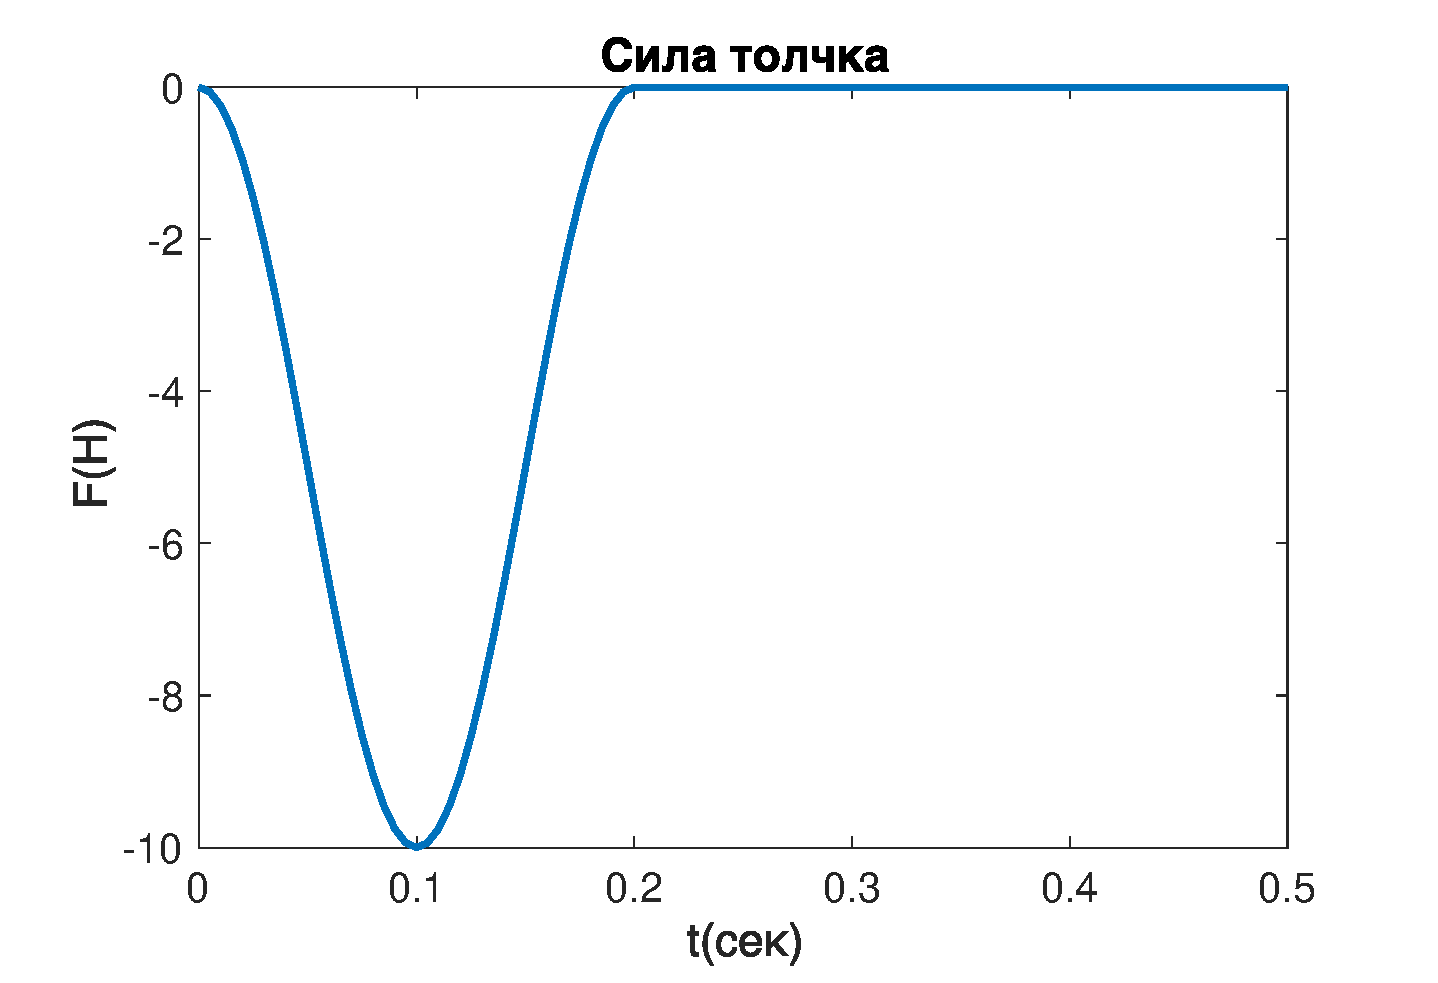
\includegraphics[width=1\linewidth]{push_model.eps}
            \caption{Пример зависимости \break $F(t)=5(1-\cos(4\pi\cdot2.5t))$}
        \end{minipage}
        \hfill
        \begin{minipage}[h]{0.48\linewidth}
            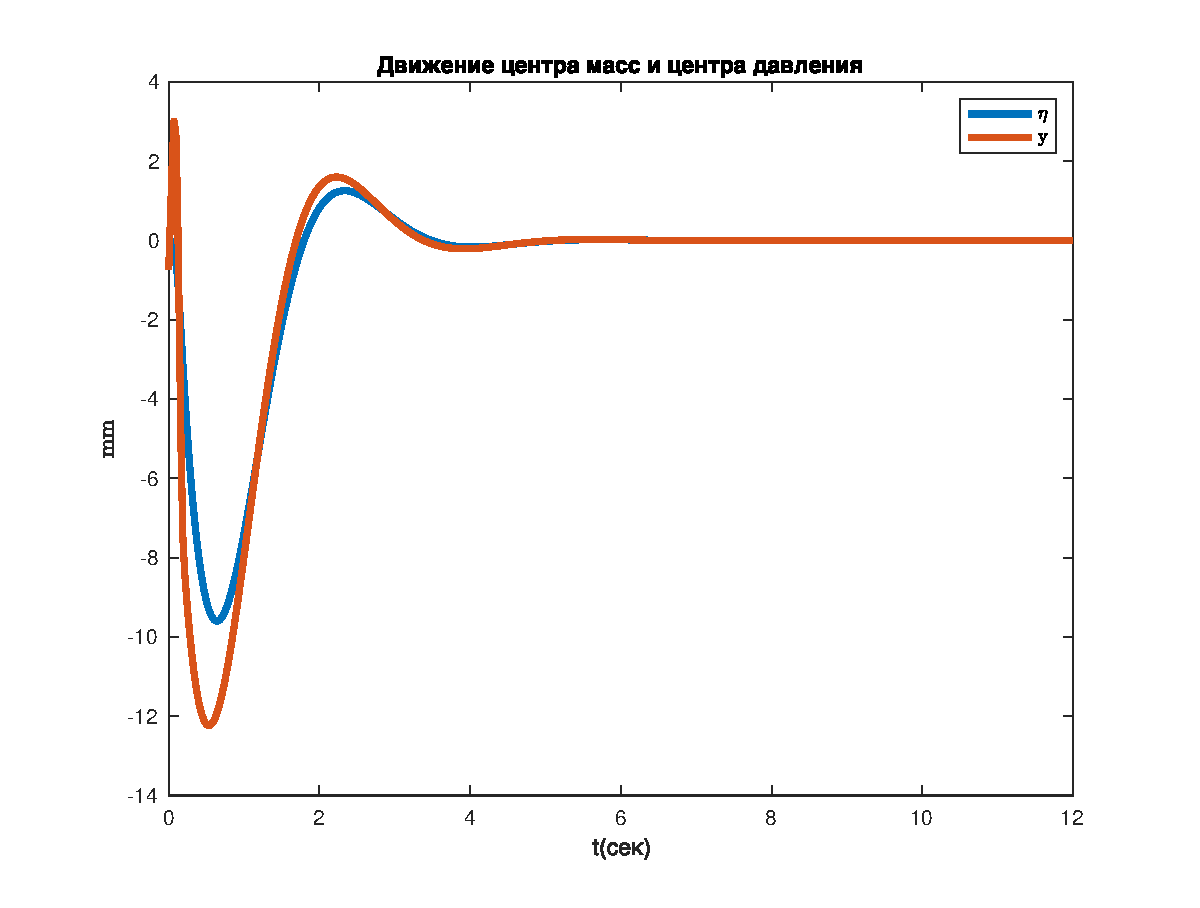
\includegraphics[width=1\linewidth]{eta_model.eps}
            \caption{Модельная траектория центра масс и центра давления}
        \end{minipage}
    \end{center}
\end{figure}

Восстановим $\eta$ двумя способами
\begin{figure}[h!]
    \begin{center}
        \begin{minipage}[h]{0.5\linewidth}
            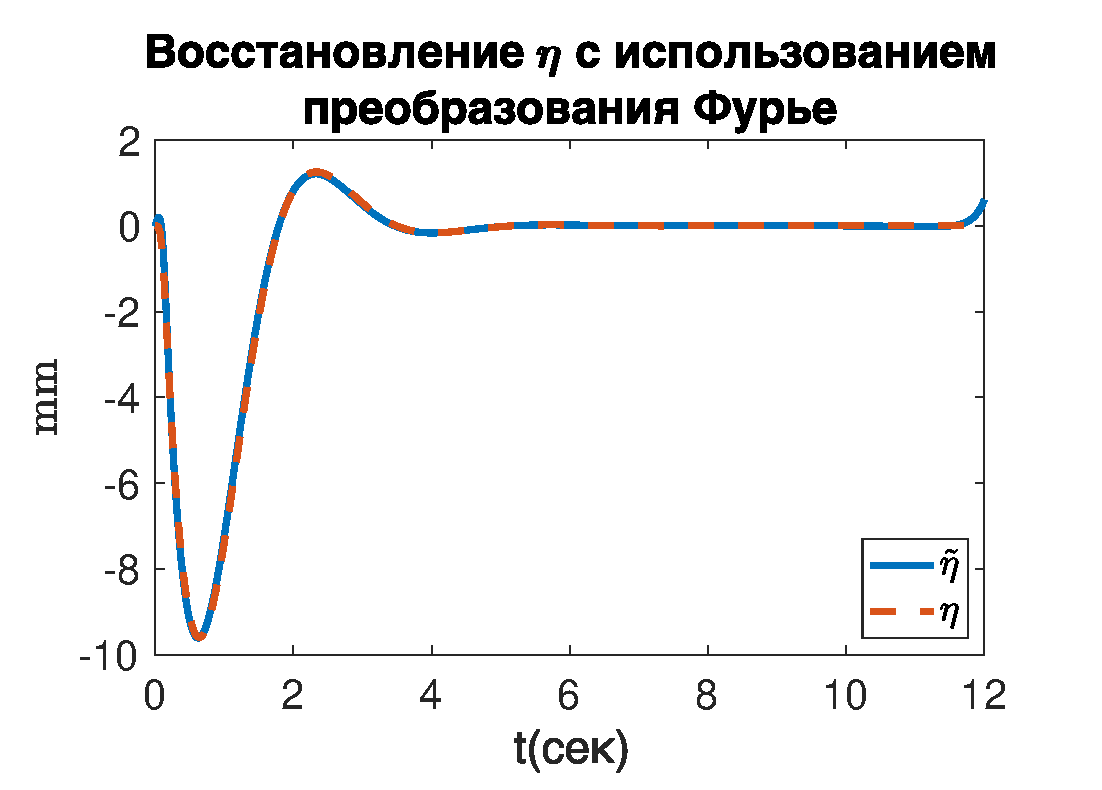
\includegraphics[width=1\linewidth]{eta_restore_fur_model.eps}
            \caption{Восстановление через преобразование Фурье}
        \end{minipage}
        \hfill
        \begin{minipage}[h]{0.48\linewidth}
            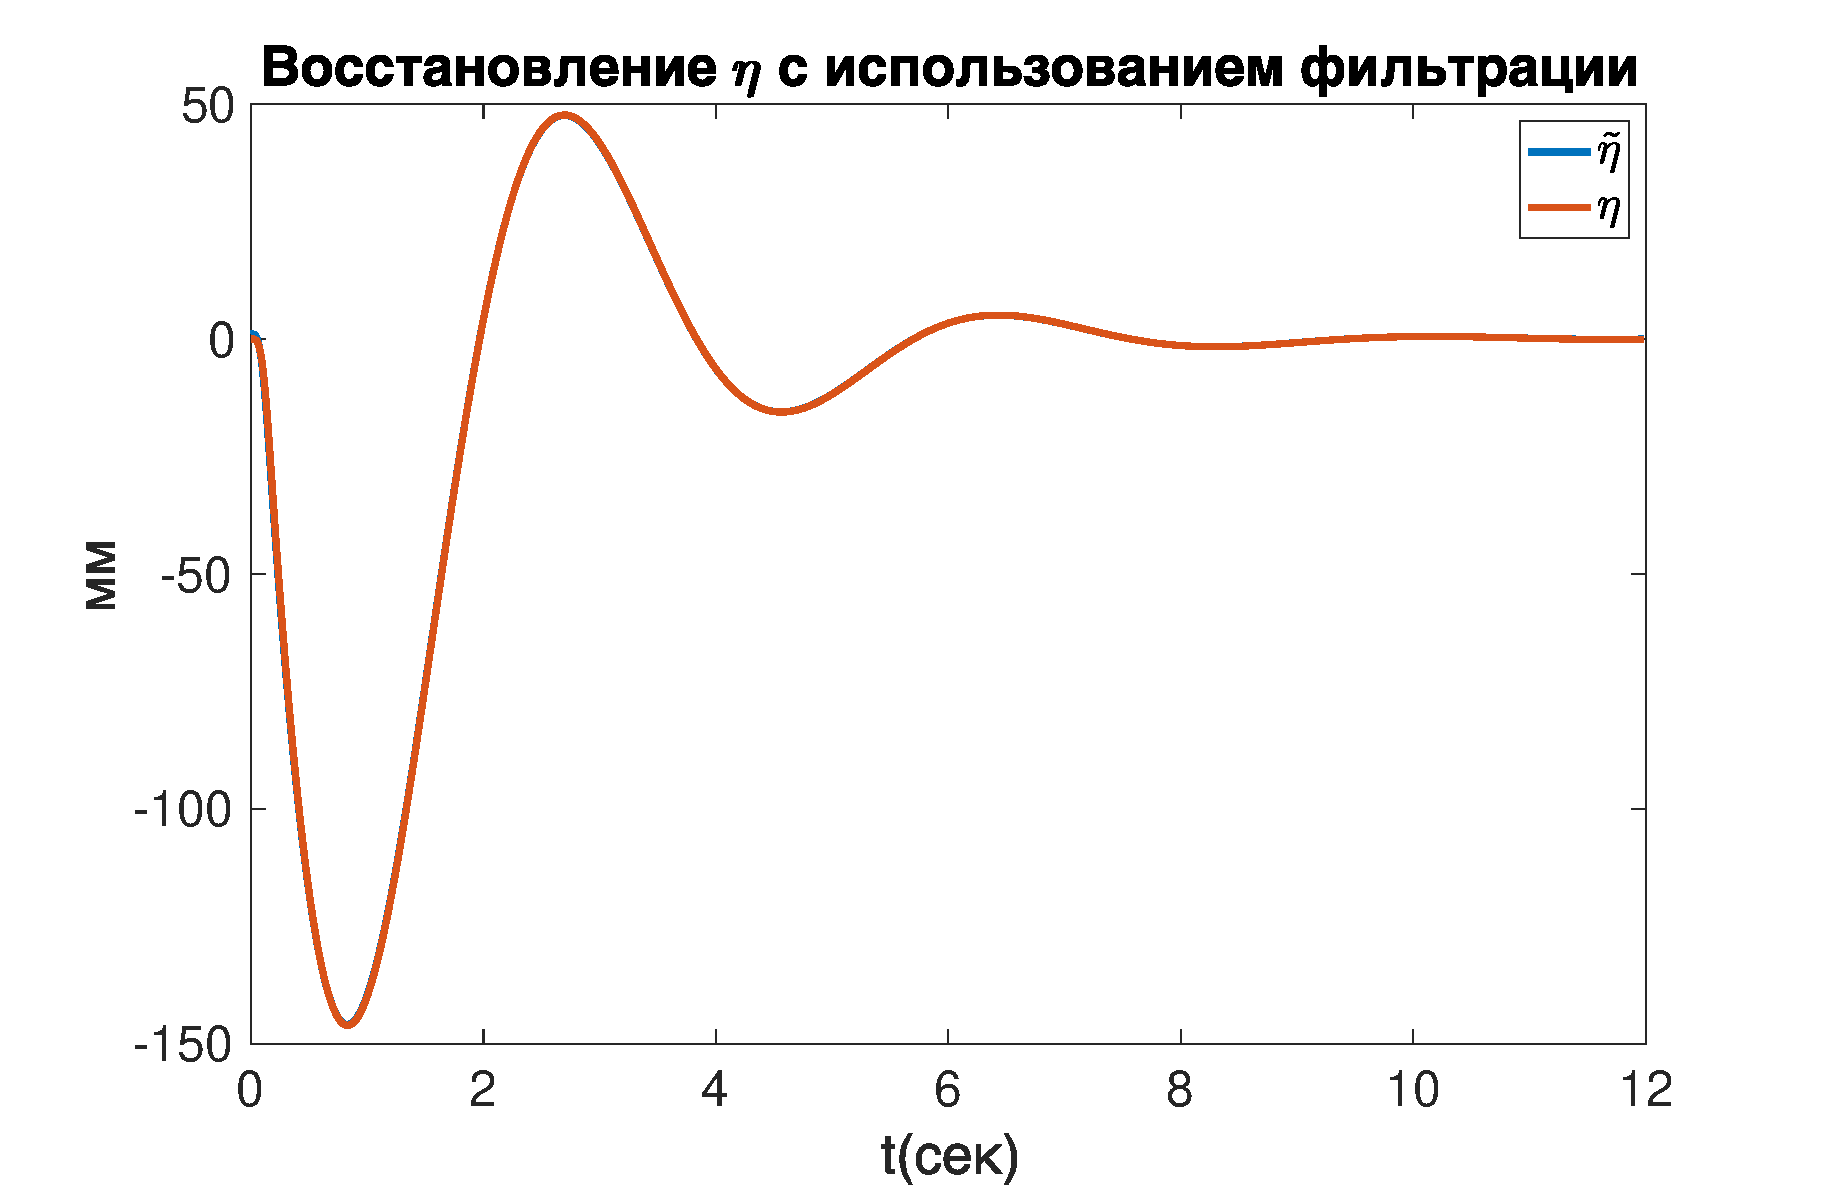
\includegraphics[width=1\linewidth]{double_filter_model.eps}
            \caption{Восстановление через двойную фильтрацию}
        \end{minipage}
    \end{center}
\end{figure}


\begin{figure}[h!]
    \begin{center}
        \begin{minipage}[h]{0.48\linewidth}
            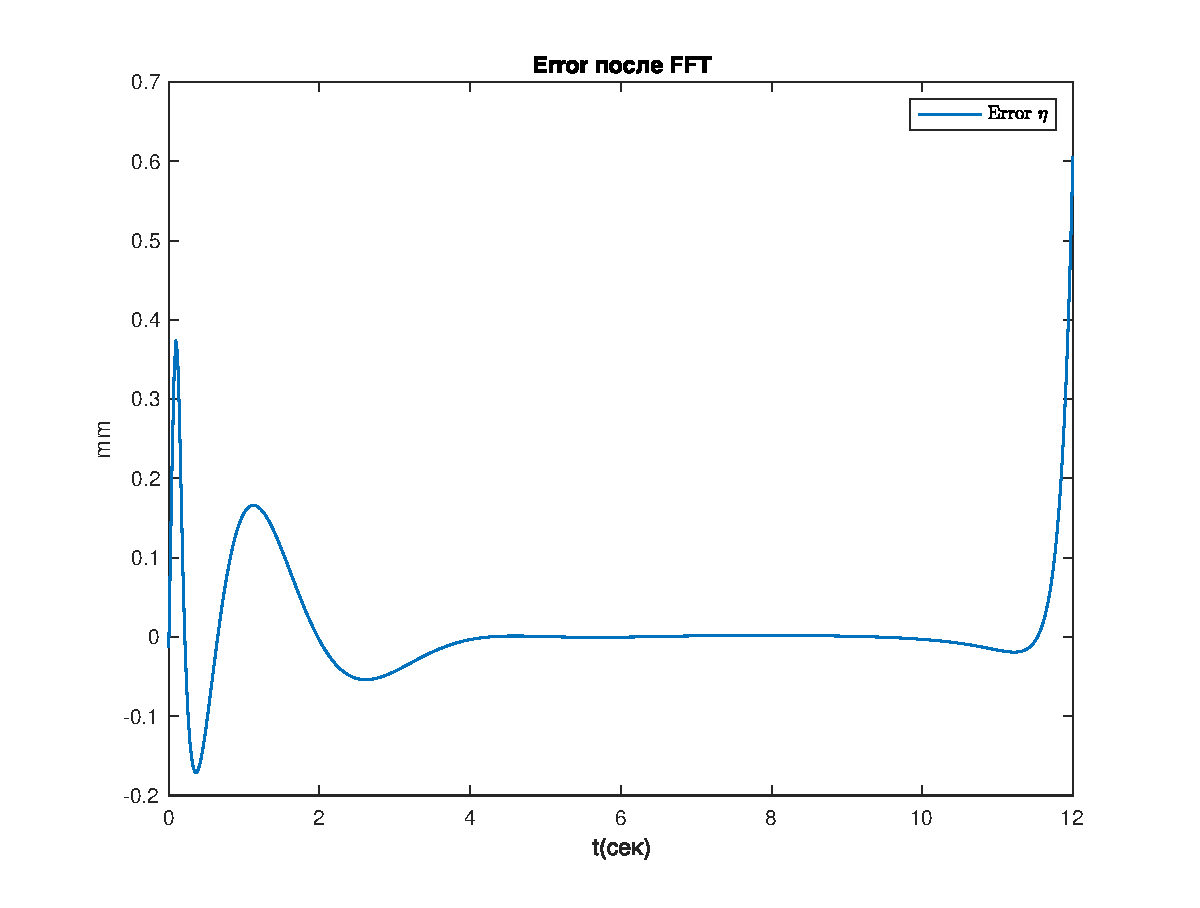
\includegraphics[width=1\linewidth]{err_furier_model.eps}
            \caption{Ошибка восстановления с использованием преобразования Фурье , $\sigma=0.076$}
        \end{minipage}
        \hfill
        \begin{minipage}[h]{0.48\linewidth}
            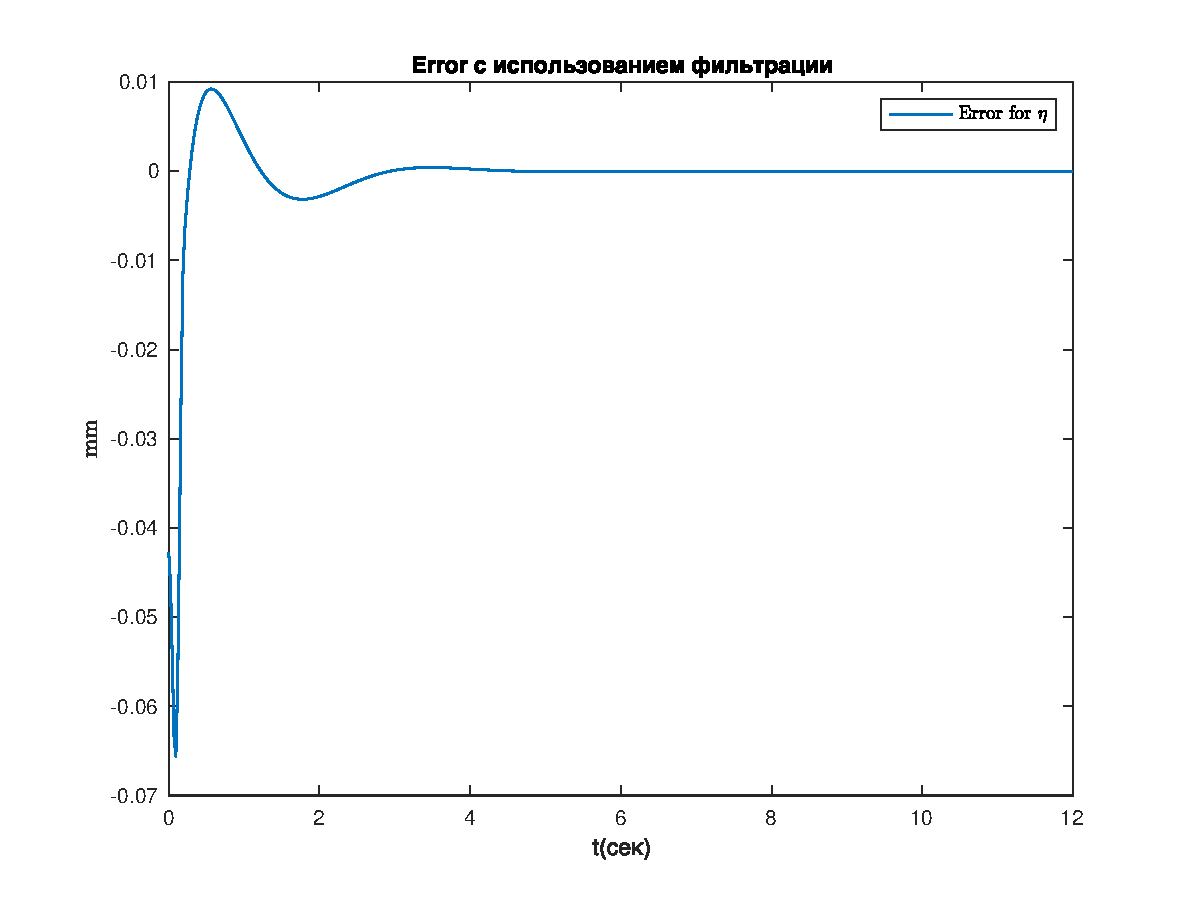
\includegraphics[width=1\linewidth]{err_double_filter_model.eps}
            \caption{Восстановление через двойную фильтрацию, $\sigma=0.006$}
        \end{minipage}
    \end{center}
\end{figure}


Погрешности обоих методов очень небольшие, почти идеально восстанавливают исходную
траекторию центра масс. Для метода, использующего Фурье преобразование
$\dfrac{\sigma}{max|\eta(t)|}=0.0079$, для двойной фильтрации $\dfrac{\sigma}{max|\eta(t)|}=0.0007$, где $\sigma-$ среднеквадратическое отклонение

\section{Анализ данных стабилоанализатора и силомера}
Оценим массу, на рисунках \ref{mass_full_time} и
\ref{mass_short_time} представлены графики показаний веса(в единицах кгс) испытуемого человека.
 На основе этих данных, путем осреденения данных на графике \ref{mass_short_time} определим $m_T -$ массу человека 

\begin{figure}[h!]
    \begin{center}
        \begin{minipage}[h]{0.49\linewidth}
            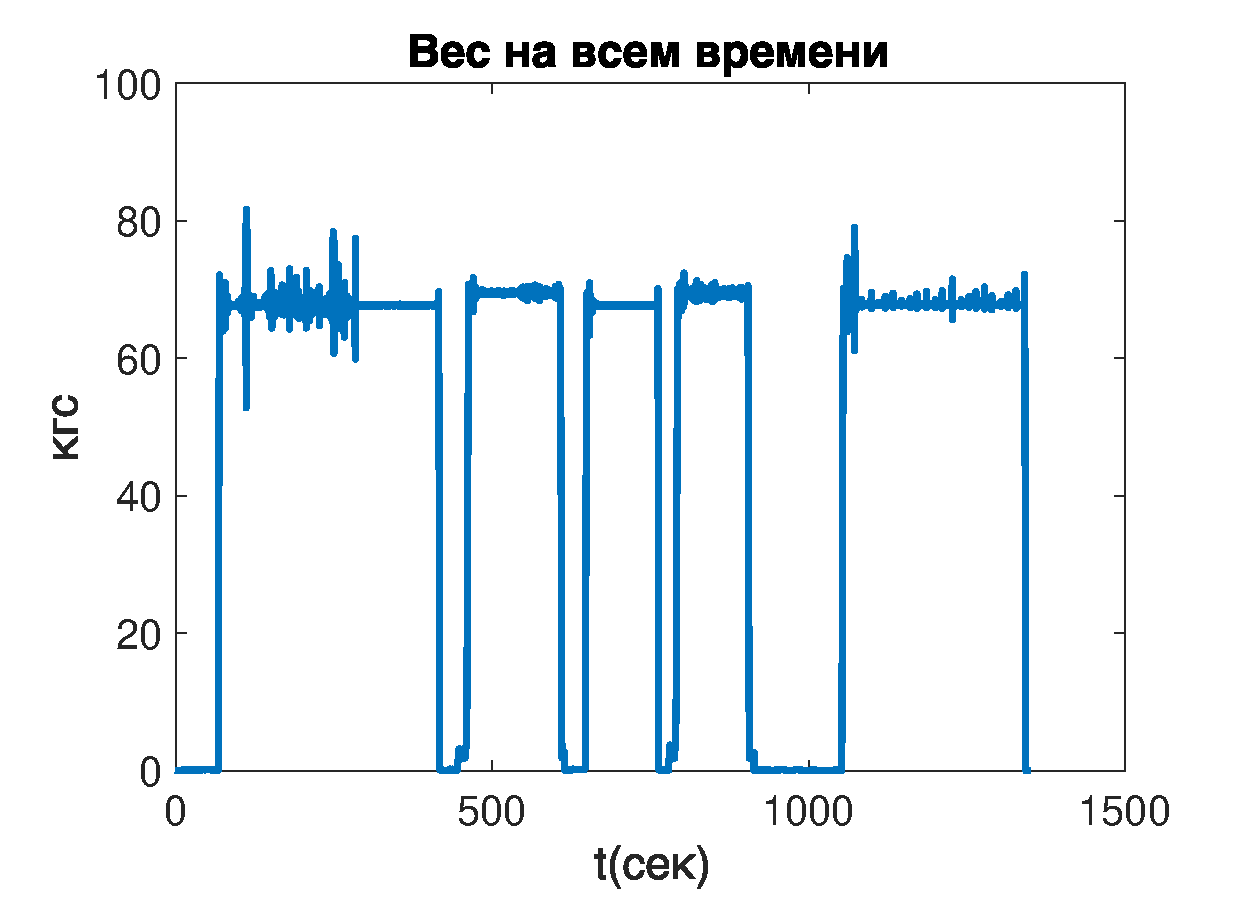
\includegraphics[width=1\linewidth]{mass_full_time.eps}
            \caption{Вес на всем интервале наблюдений}
            \label{mass_full_time}
        \end{minipage}
        \hfill
        \begin{minipage}[h]{0.49\linewidth}
            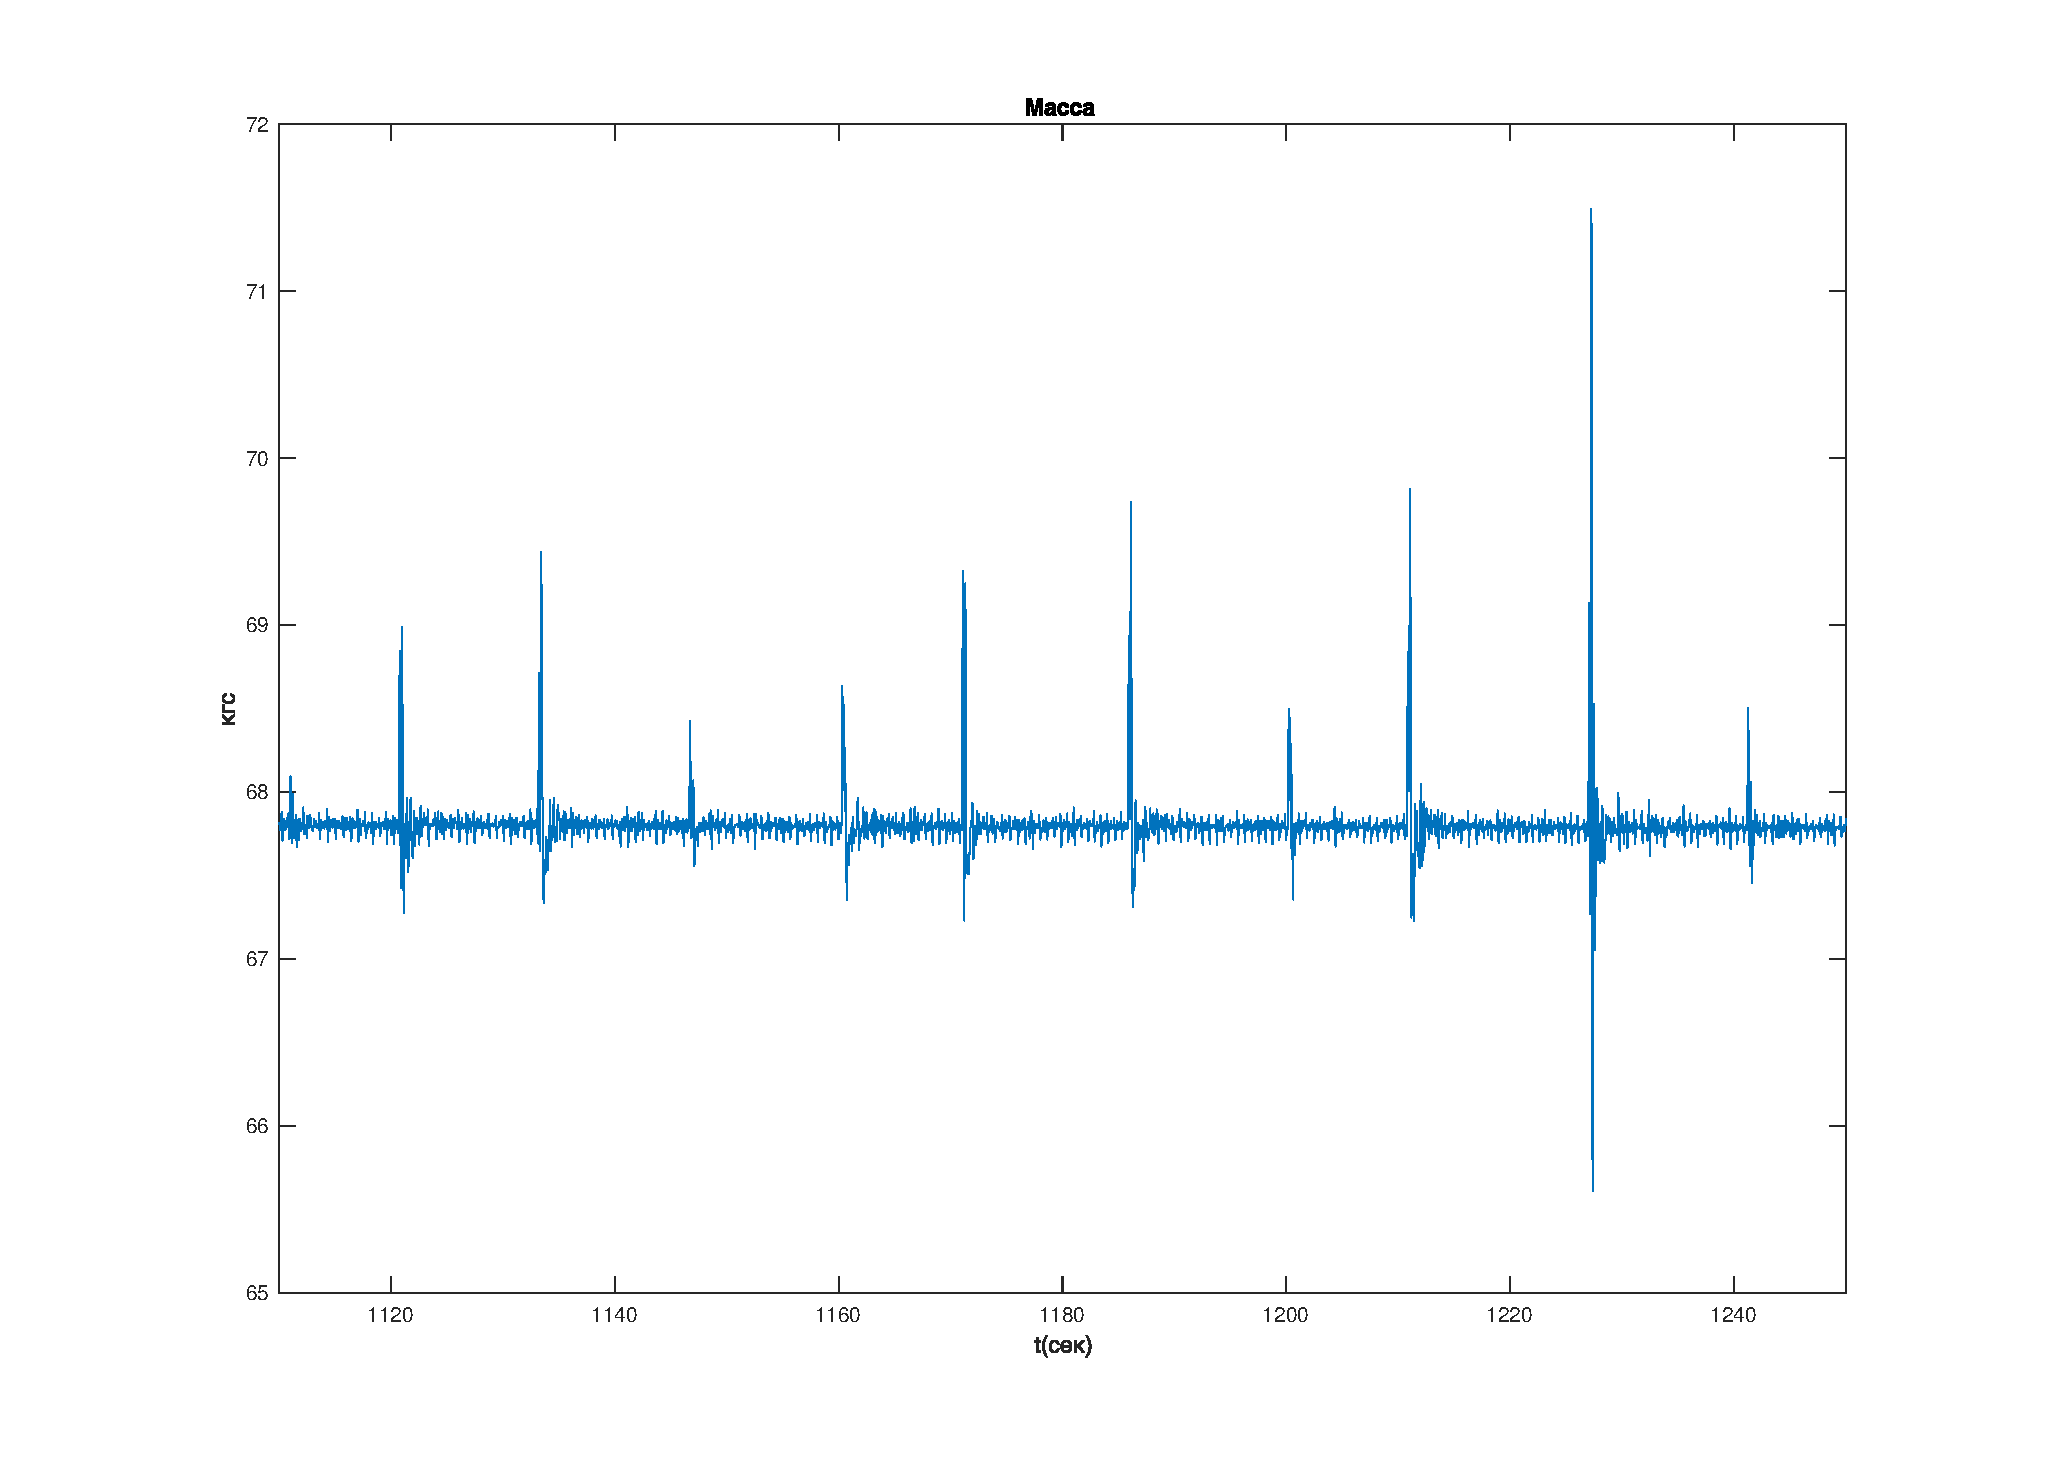
\includegraphics[width=1\linewidth]{mass_concrete.eps}
            \caption{Вес на интервале толчков}
            \label{mass_short_time}
        \end{minipage}
    \end{center}
\end{figure}

$m_T=67.8$кг

Проанализируем силу толчков (см. рис. \ref{pushes_real}), сила толчка колеблется от 1 до 10 Н,
в первую очередь возьмем толчки большей силы, так как на них предположительно лучше удастся провести исследование.

\begin{figure}[h!]
    \centering
    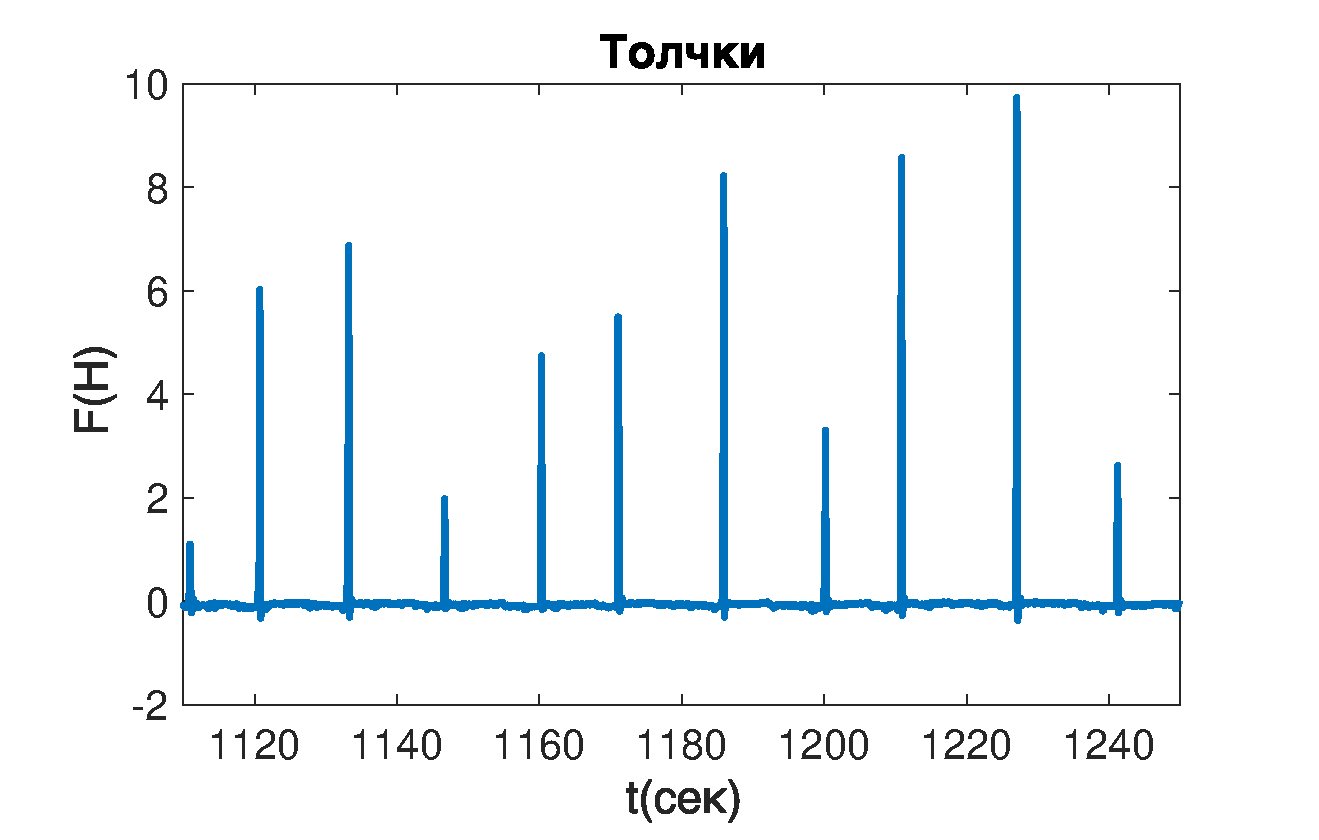
\includegraphics[width=0.9\linewidth]{pushes_real.eps}
    \caption{Силовое воздействие на интервале наблюдения}
    \label{pushes_real}
\end{figure}

\begin{figure}[h!]
    \centering
    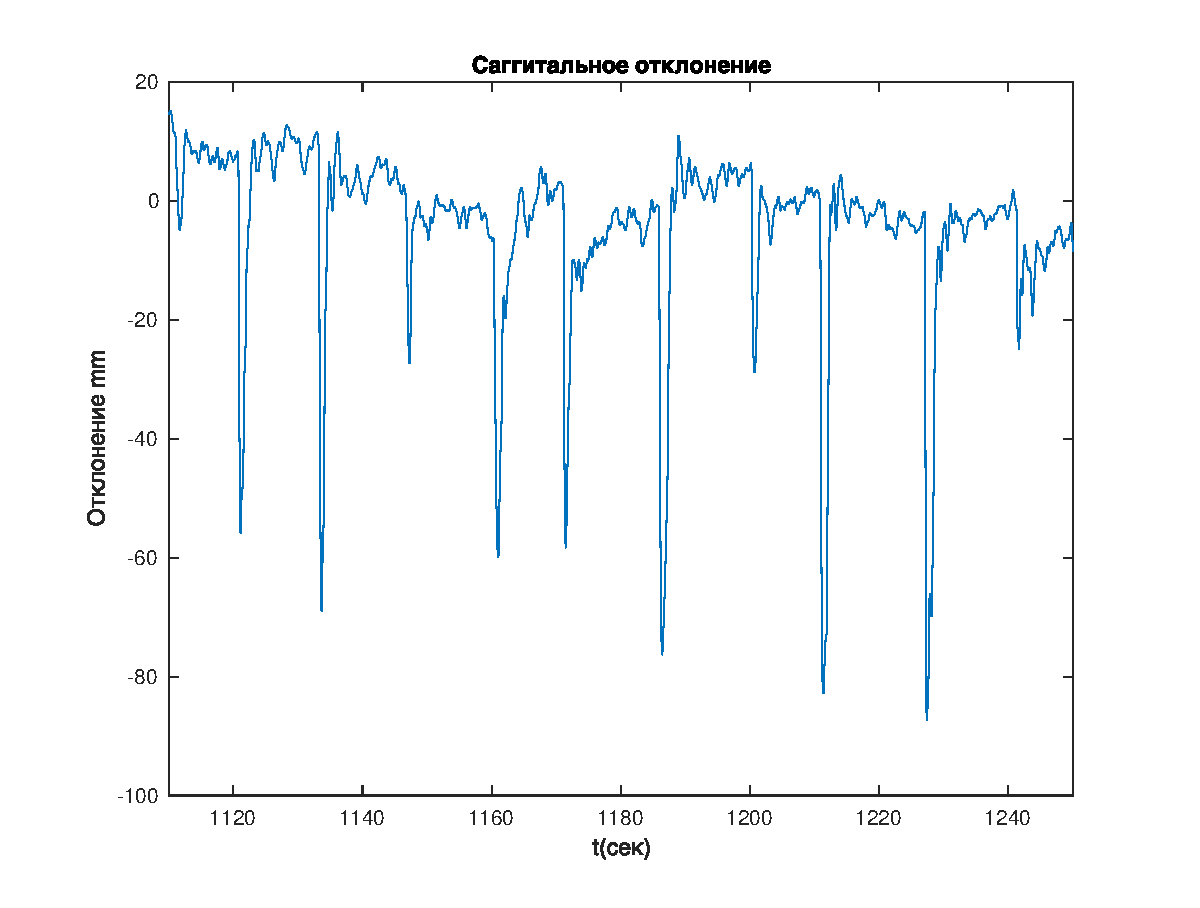
\includegraphics[width=0.9\linewidth]{y_real.eps}
    \caption{Саггитальное отклонение центра давления при толчках}
    \label{y_real}
\end{figure}



\section{Применение алгоритмов фильтрации к экспериментальным данным}
Рассмотрим для примера первый толчок (около момента времени 1120) и для него применим два способа
фильтрации (см. рис. \ref{restore_double_real} и \ref{restore_fur_real}), для того, 
чтобы оценить какой из них лучше подходит для наших данных.

\begin{figure}[h!]
    \centering
    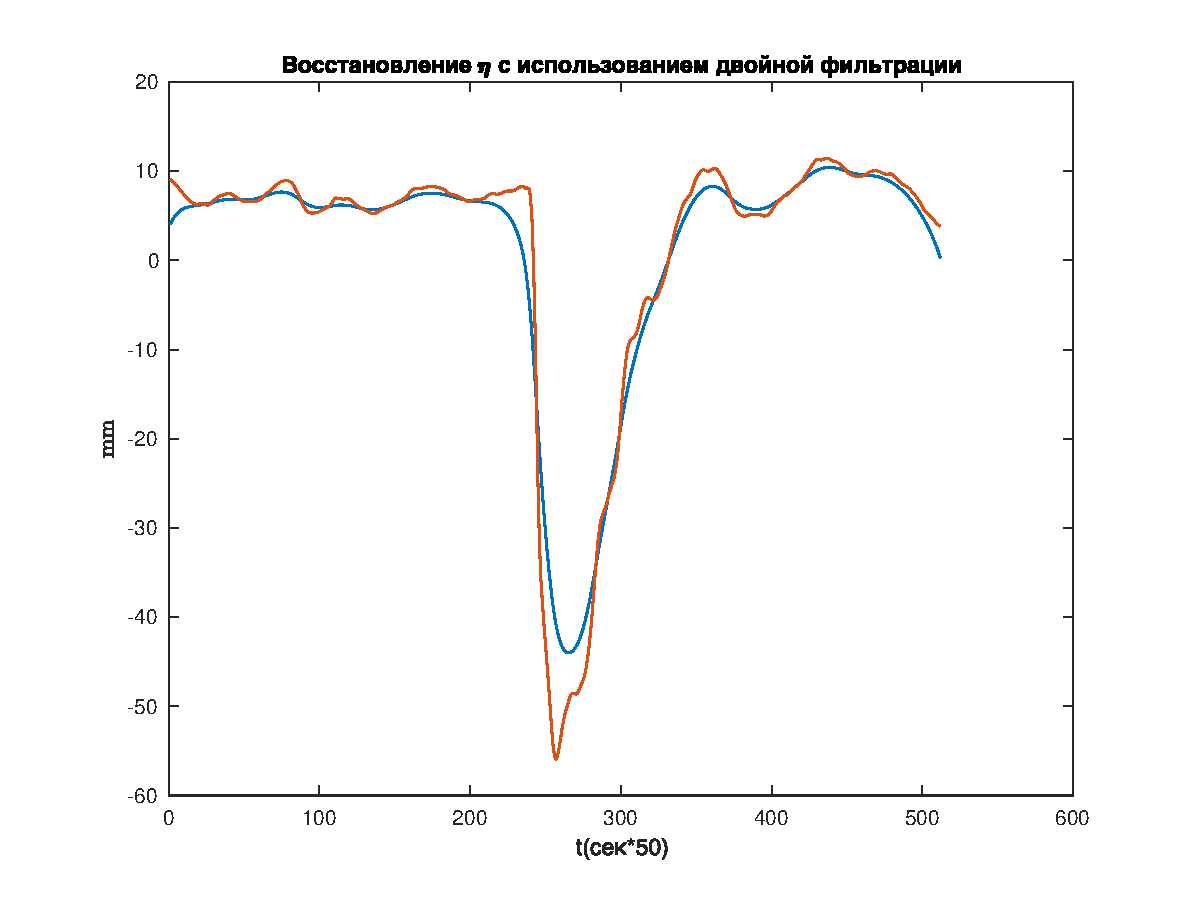
\includegraphics[width=0.9\linewidth]{restore_eta_double_real.eps}
    \caption{Восстановление с использованием двойной фильтрации $\sigma=7.9$}
    \label{restore_double_real}
\end{figure}

\begin{figure}[h!]
    \centering
    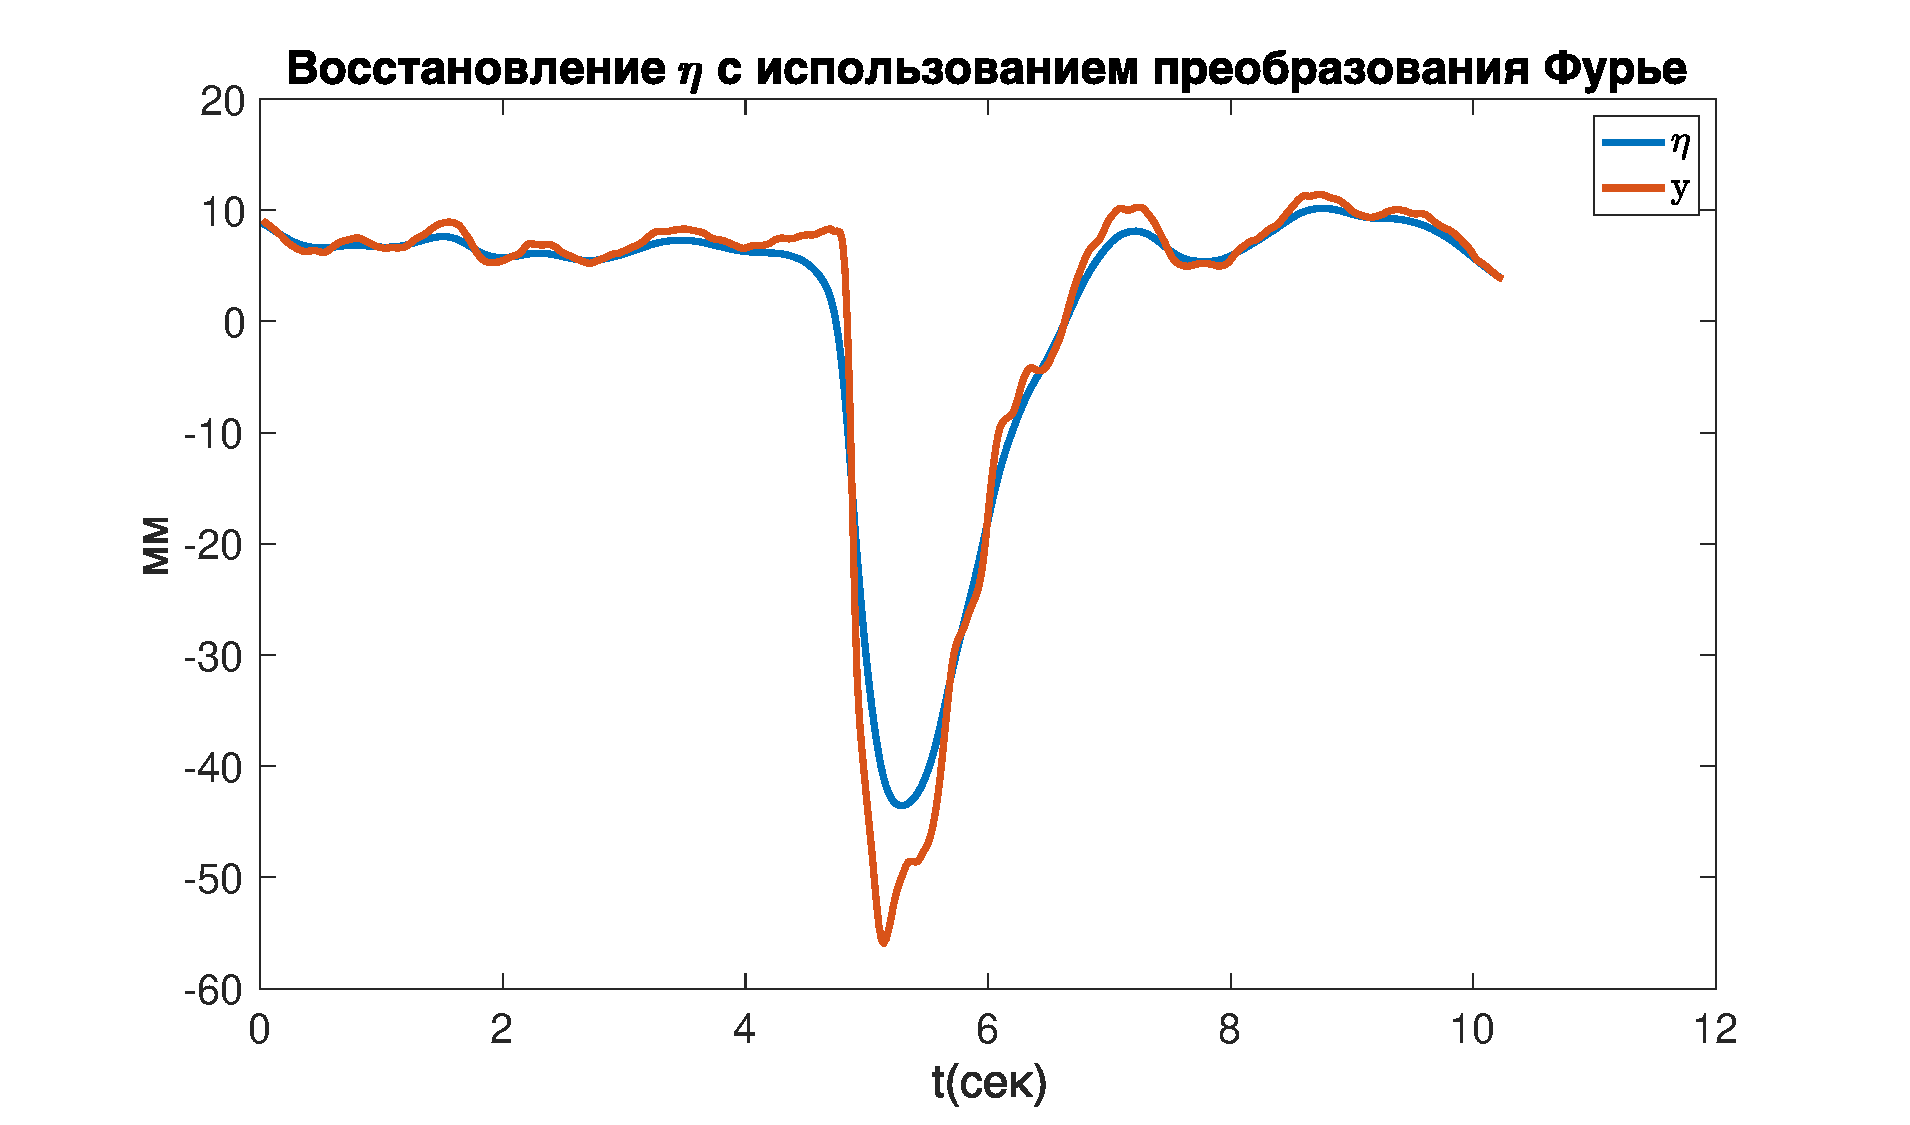
\includegraphics[width=0.9\linewidth]{restore_eta_fur_real.eps}
    \caption{Восстановление с использованием преобразования Фурье $\sigma=3.0$}
    \label{restore_fur_real}
\end{figure}

Отношение, $\dfrac{\sigma}{max|\eta(t)|}$ примерно равно $0.07$ для обоих методов, полученная траектории центра масс и исходная траектория 
центра давления довольно близки. Для дальнейшего анализ будем использовать метод двойной фильтрации, 
так как на модельных данных он дал меньшую погрешность восстановления $\tilde{\eta}$.

\section{Оценка неизвестных параметров задачи}

В задаче быстродейтсвия присутсвует несколько неизвестных параметров:

$u_*$ - модуль оптимального управления,
$t_*$ - коэффицент обезразмеривания времени,
$\varphi_*\approx\varphi_0$ - характерное значение угла отклонения тела


$l=0.88$м

$$t_\ast=\sqrt{\frac{J}{m_Tgl}}=\sqrt{\frac{1/3 \cdot m_T l^2}{m_Tgl}}=\sqrt{\frac{l}{3g}}$$
\[
    u^-=\frac{t_\ast U^-}{m_Tgl\varphi_\ast },\ \ u^+=\frac{t_\ast U^+}{m_Tgl\varphi_\ast}.
\]
$|U^+|=|U^-|=\dot M\approx \Delta M \cdot \nu, \text{ где } \nu - \text{частота дискретизации данных на стабилоанализаторе } $
$\nu =50\text{Гц}$

В работе \cite{kruchinMetoda} показано, что $\Delta y\approx\dfrac{\Delta M}{m_Tg}$.

Возьмем 5 толчков и по ним определим средний возникающий момент в голеностопе см. таблицу \ref*{moments_calculating}

tНачало - время когда начался толчок

tКонец - время когда, началось возвратное движение центра давления

$\Delta y - $ изменение центра давления за время $\Delta t = $tКонец-tНачало

$\Delta M - $ момент в голеностопе, возникший за время $\Delta t$
\begin{table}[h!]
    \centering
    \begin{tabular}{|l|c|c|c|c|}
        \hline
        \textbf{}                                    &
        \multicolumn{1}{l|}{\textbf{tНачало(сек)}}    &
        \multicolumn{1}{l|}{\textbf{tКонец(сек)}}      &
        \multicolumn{1}{l|}{\textbf{$\Delta y$(мм)}} &
        \multicolumn{1}{l|}{\textbf{$\Delta M $(Н $\cdot$ м)}}                        \\ \hline
        \textbf{1}                                   & 1098.9 & 1099.3 & 64.7  & 43.1 \\ \hline
        \textbf{2}                                   & 1120.8 & 1121.0 & 61.5  & 40.9 \\ \hline
        \textbf{3}                                   & 1133.2 & 1133.6 & 72.6  & 48.3 \\ \hline
        \textbf{4}                                   & 1185.9 & 1186.2 & 65.18 & 43.4 \\ \hline
        \textbf{5}                                   & 1277.8 & 1278.0 & 67.3  & 44.7 \\ \hline
    \end{tabular}
    \caption{Данные для расчета возникающего момента в голеностопе, см. рис. \ref{y_real} }
    \label{moments_calculating}
\end{table}

Среднее значение $\Delta M=44.0$ Н$\cdot$м

$\max(\Delta M)=48.3$ Н$\cdot$м

$\min(\Delta M)=40.9$ Н$\cdot$м

Среднее значение $U^+=\dfrac{\Delta M}{\Delta t}=144.7$ Н$\cdot$м/c $,\Delta t_i=xEnd_i-xStart_i$
\begin{figure}[h!]
    \centering
    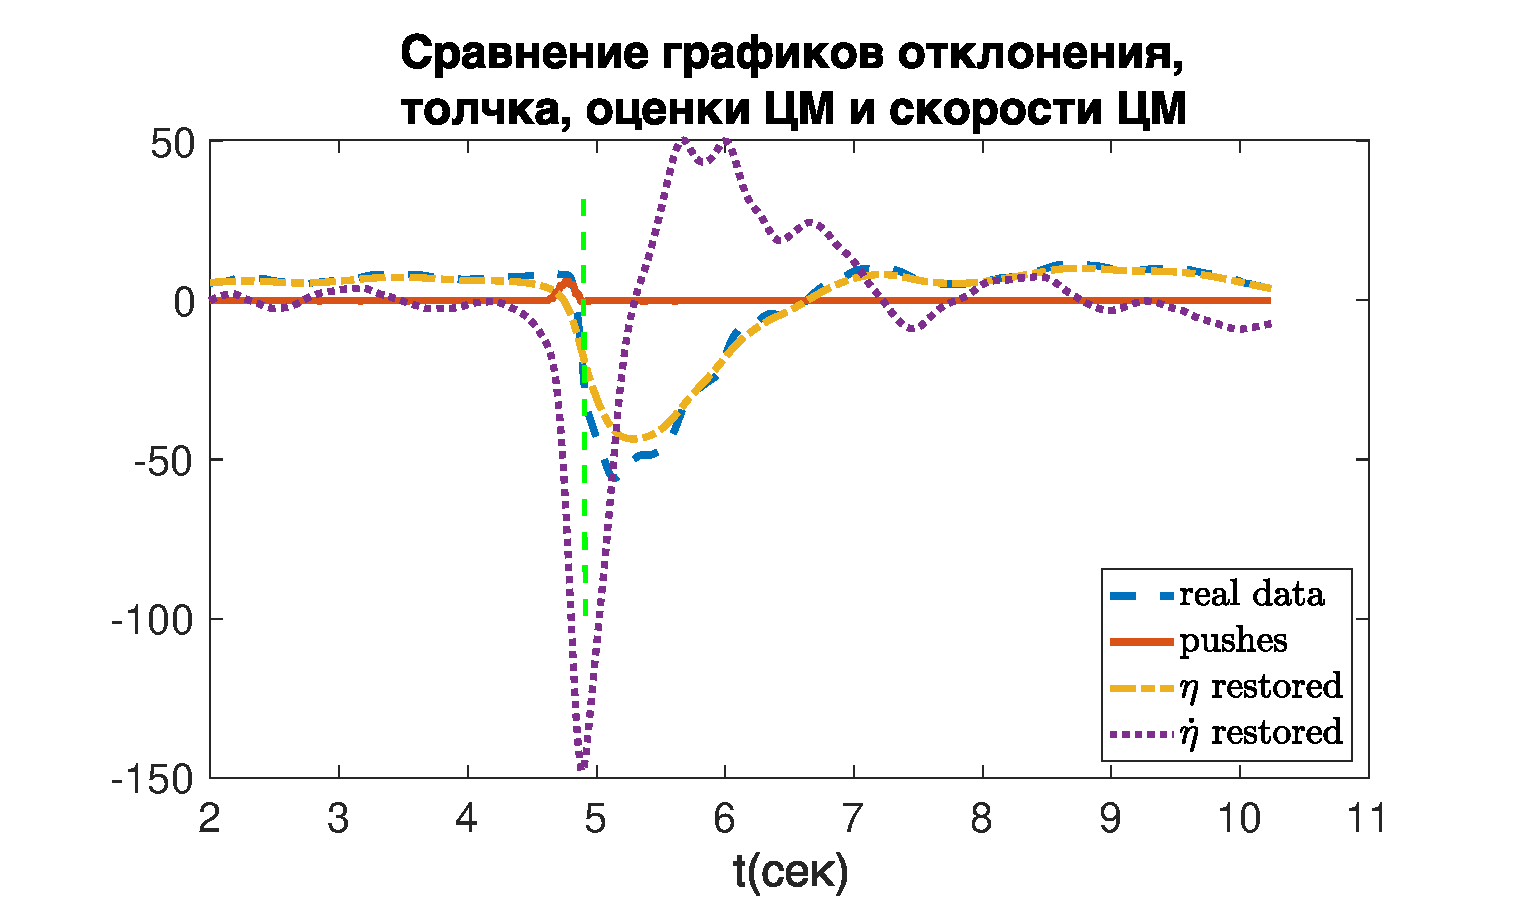
\includegraphics[width=0.99\linewidth]{cp3_bold.eps}
    \caption{К определению начальных условий в момент завершения толчка}
    \label{all_real}
\end{figure}

На рисунке \ref{all_real} представлены графики исходных данных(пунктирная), данные силомера(сплошная), траектория центра масс(штрих-пунктирная), восстановленная с помощью метода двойной фильтрации и ее первая производная(точечная), вычисленная как первая разность, умноженная на частоту дискретизации.

Вертикальная ось - Н, мм, мм/с для соответствующих величин. Момент завершения толчка соответствует
 моменту времени, отмеченному вертикальной пунктирной линией с абсциссой $t=245\left( \dfrac{c}{50} \right)$. В ней берем начальные условия:

$$\varphi_0=-\dfrac{\tilde{\eta}(245)}{l}\cdot\dfrac{1}{1000}=0.0292\text{ рад}$$

$$\omega_0=-\dfrac{\dot{\tilde{\eta}}(245)}{l}\cdot\dfrac{1}{1000}=0.1490\text{ рад/с}$$

Коэффицент $\dfrac{1}{1000}$ нужен для преобразования миллиметров в метры.

Посчитаем безразмерное $u_\ast$

\[
    u_\ast=\frac{t_\ast U^-}{m_Tgl\varphi_\ast }=1.46
\]


\newpage

\chapter{Анализ полученных решений задачи быстродействия}

\section{Сравнение траекторий и времени возвращения для выборки толчков}


При $u_\ast=1.46$ действительных корней уравнения \eqref{final_polynom} больших 1 нет,
при обоих комбинациях знаков $u_\ast$.

Объяснение этому явлению такое (см. рис. \ref{all_bold}): в реальности в голеностопе уже возник некоторый возвращающий момент, за счет нервной системы и быстрореагирующих мышечных волокн,
 который возникает в результате реакции на изменение длины мышцы.
В принятой в исследовании постановке задачи, считается, что момент не успел возникнуть. Для корректировки завысим значение $u_\ast$ в $2-3$ раза.
\begin{figure}[h!]
    \centering
    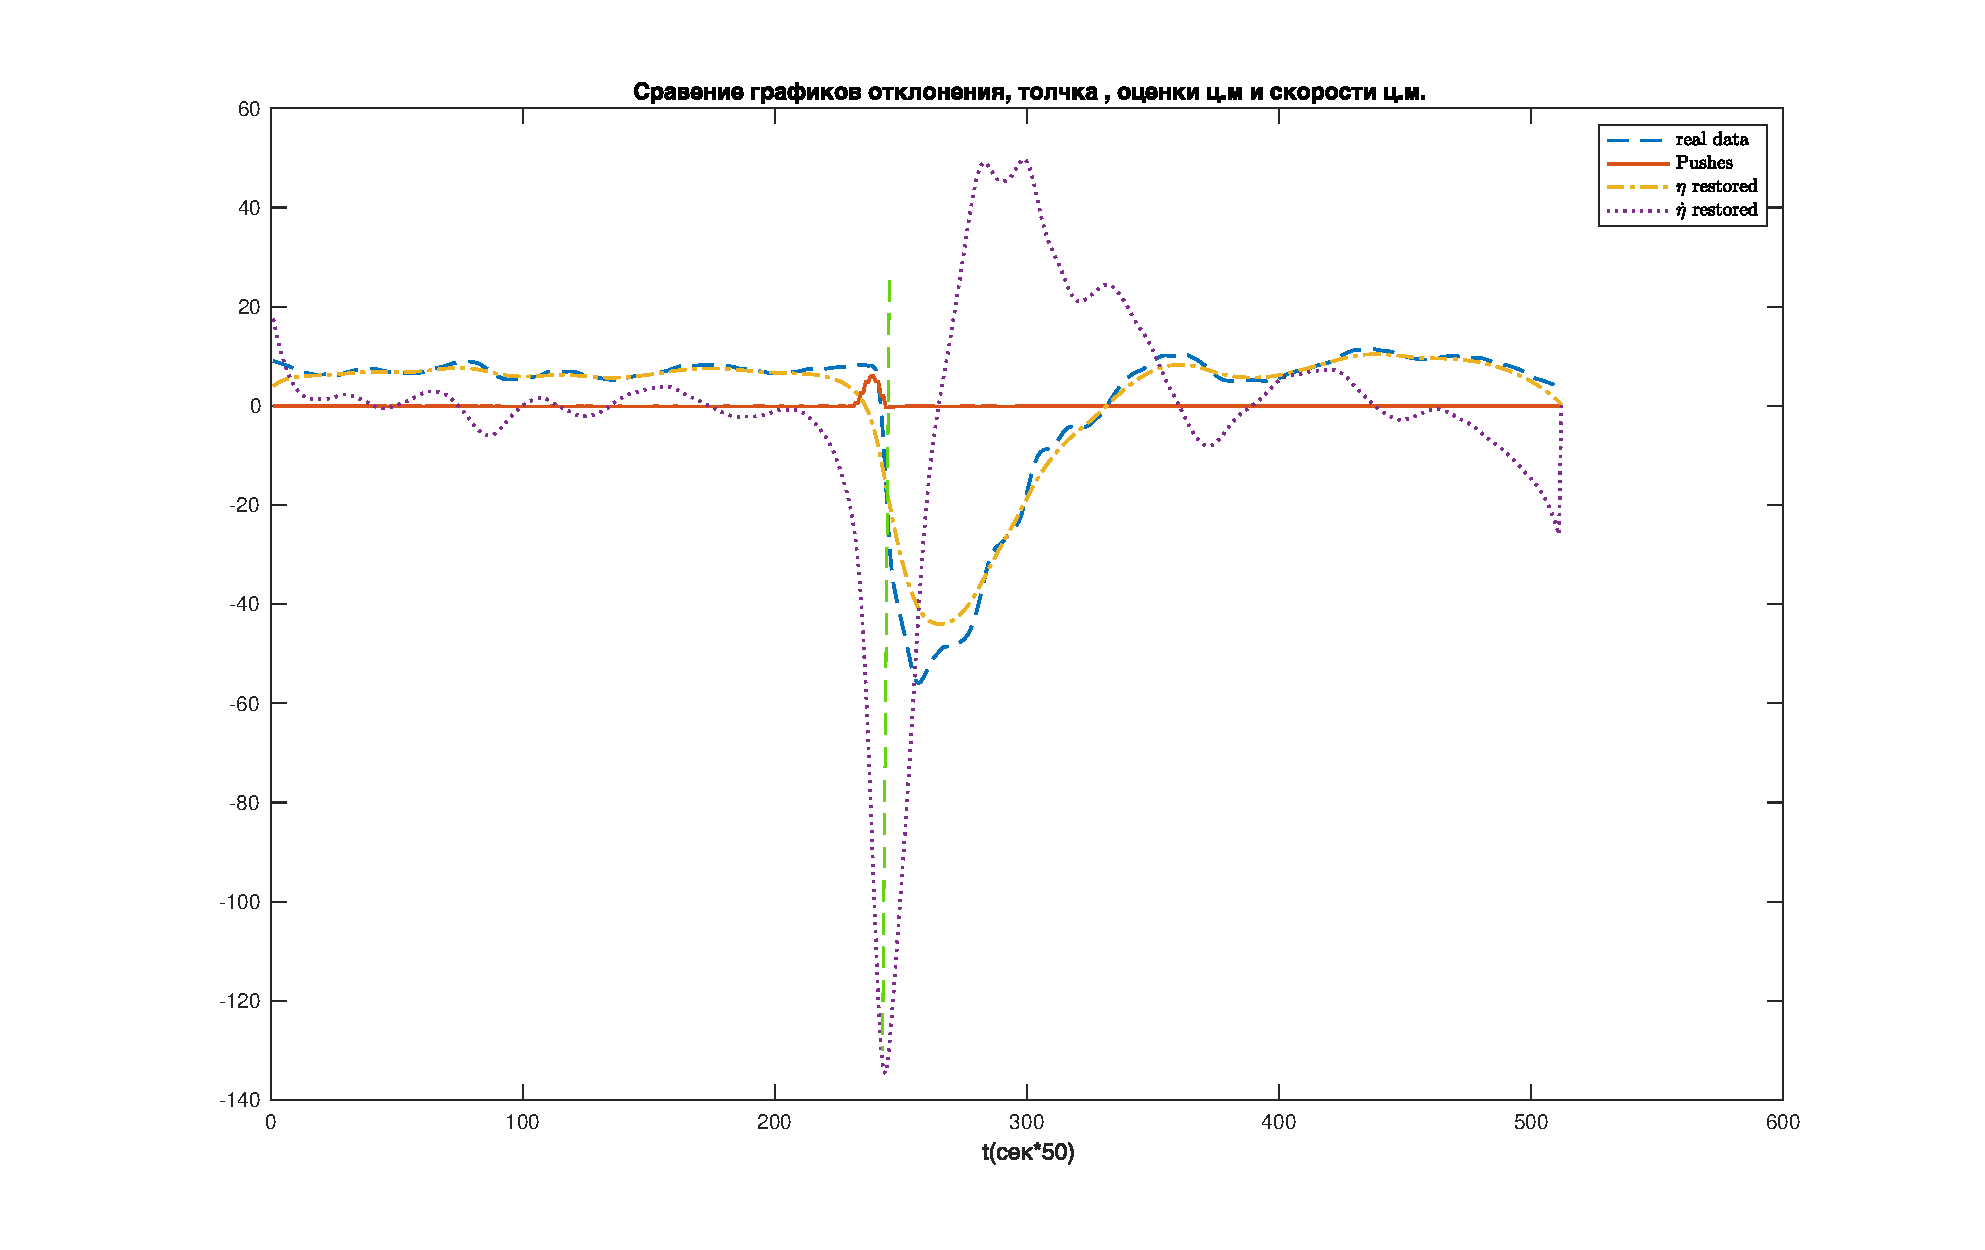
\includegraphics[width=0.9\linewidth]{all_real.eps}
    \caption{К объяснению возникновения начального ненулевого момента}
    \label{all_bold}
\end{figure}
\begin{figure}[h!]
    \centering
    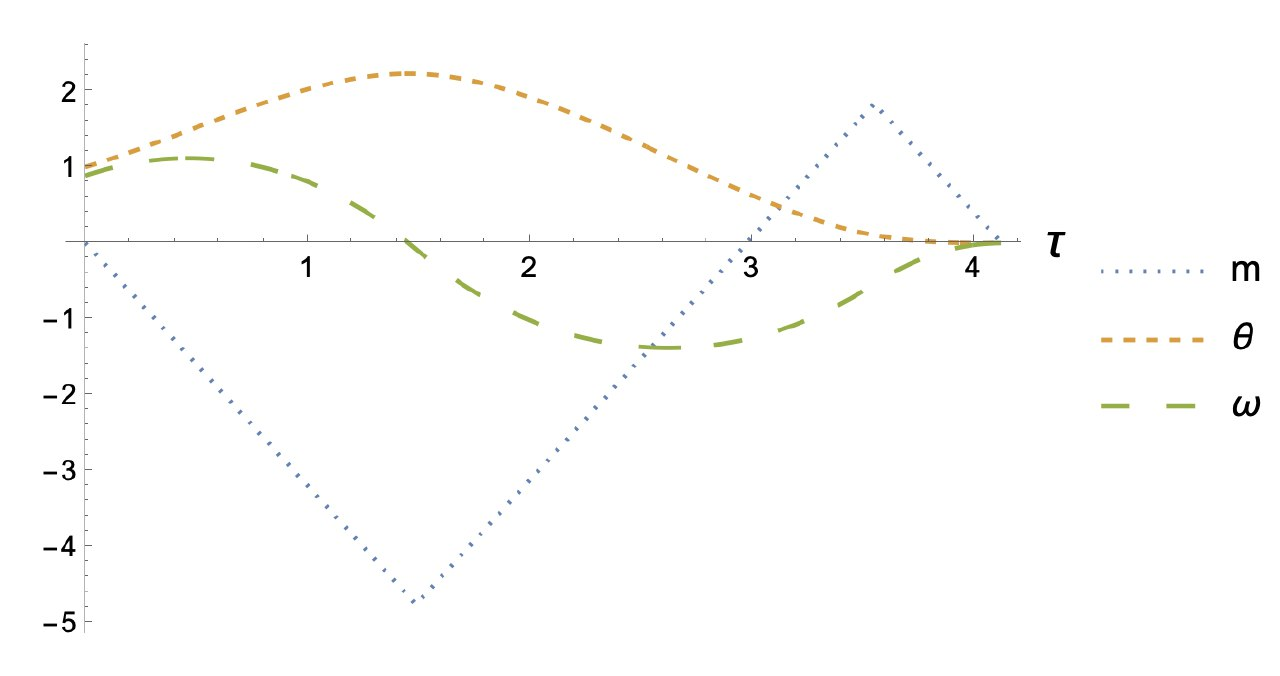
\includegraphics[width=0.9\linewidth]{3_graphs.jpeg}
    \caption{Оптимальная траектории в безразмерном виде $u=3.2$ }
    \label{3_graphs}
\end{figure}

Посторим полученные траектории для различных значений $u_\ast$(см. рис. \ref{final_graphs}, \ref{final_graphs_1}).

Траектория центра масс содержит смещения относительно нуля, поэтому примем за ноль положение спокойного стояния.

\begin{figure}[h!]
    \centering
    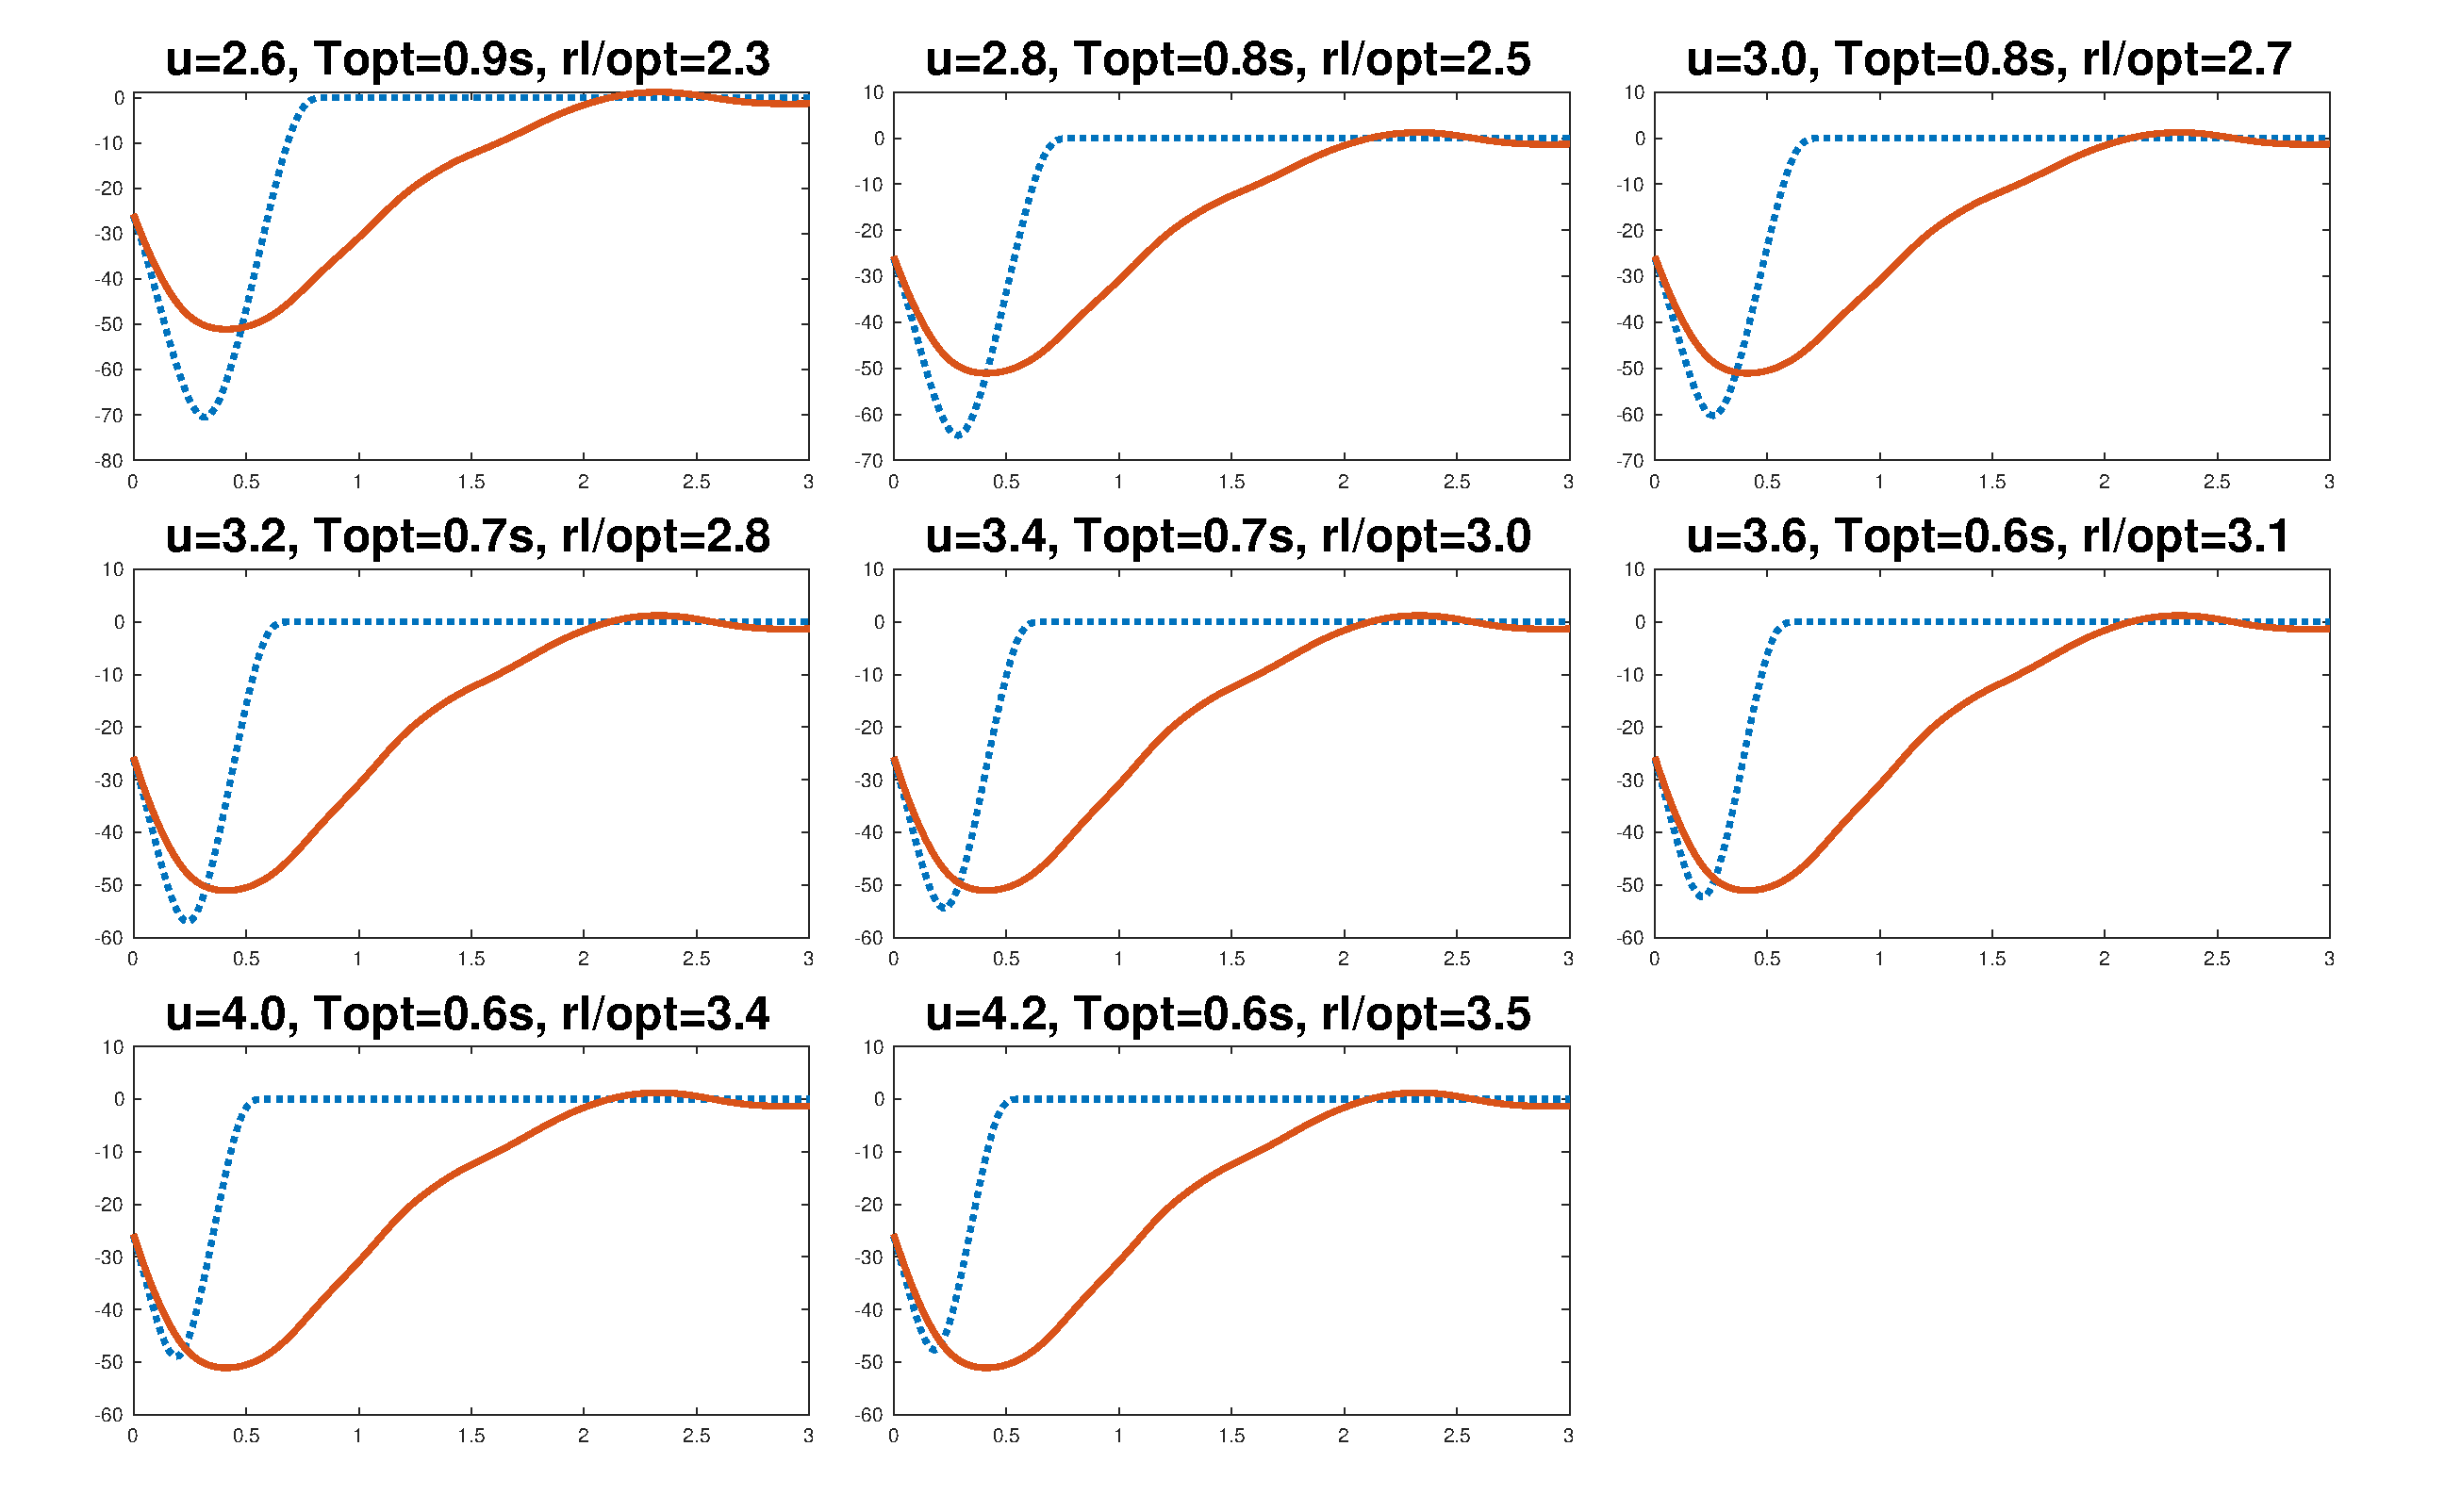
\includegraphics[width=1\linewidth]{final_graphs.eps}
    \caption{Сравнение характерных оптимальных(пунктирные) и реальных(сплошные) траектории на возвратном движении человека $t=1120$}
    \label{final_graphs}
\end{figure}

\begin{figure}[h!]
    \centering
    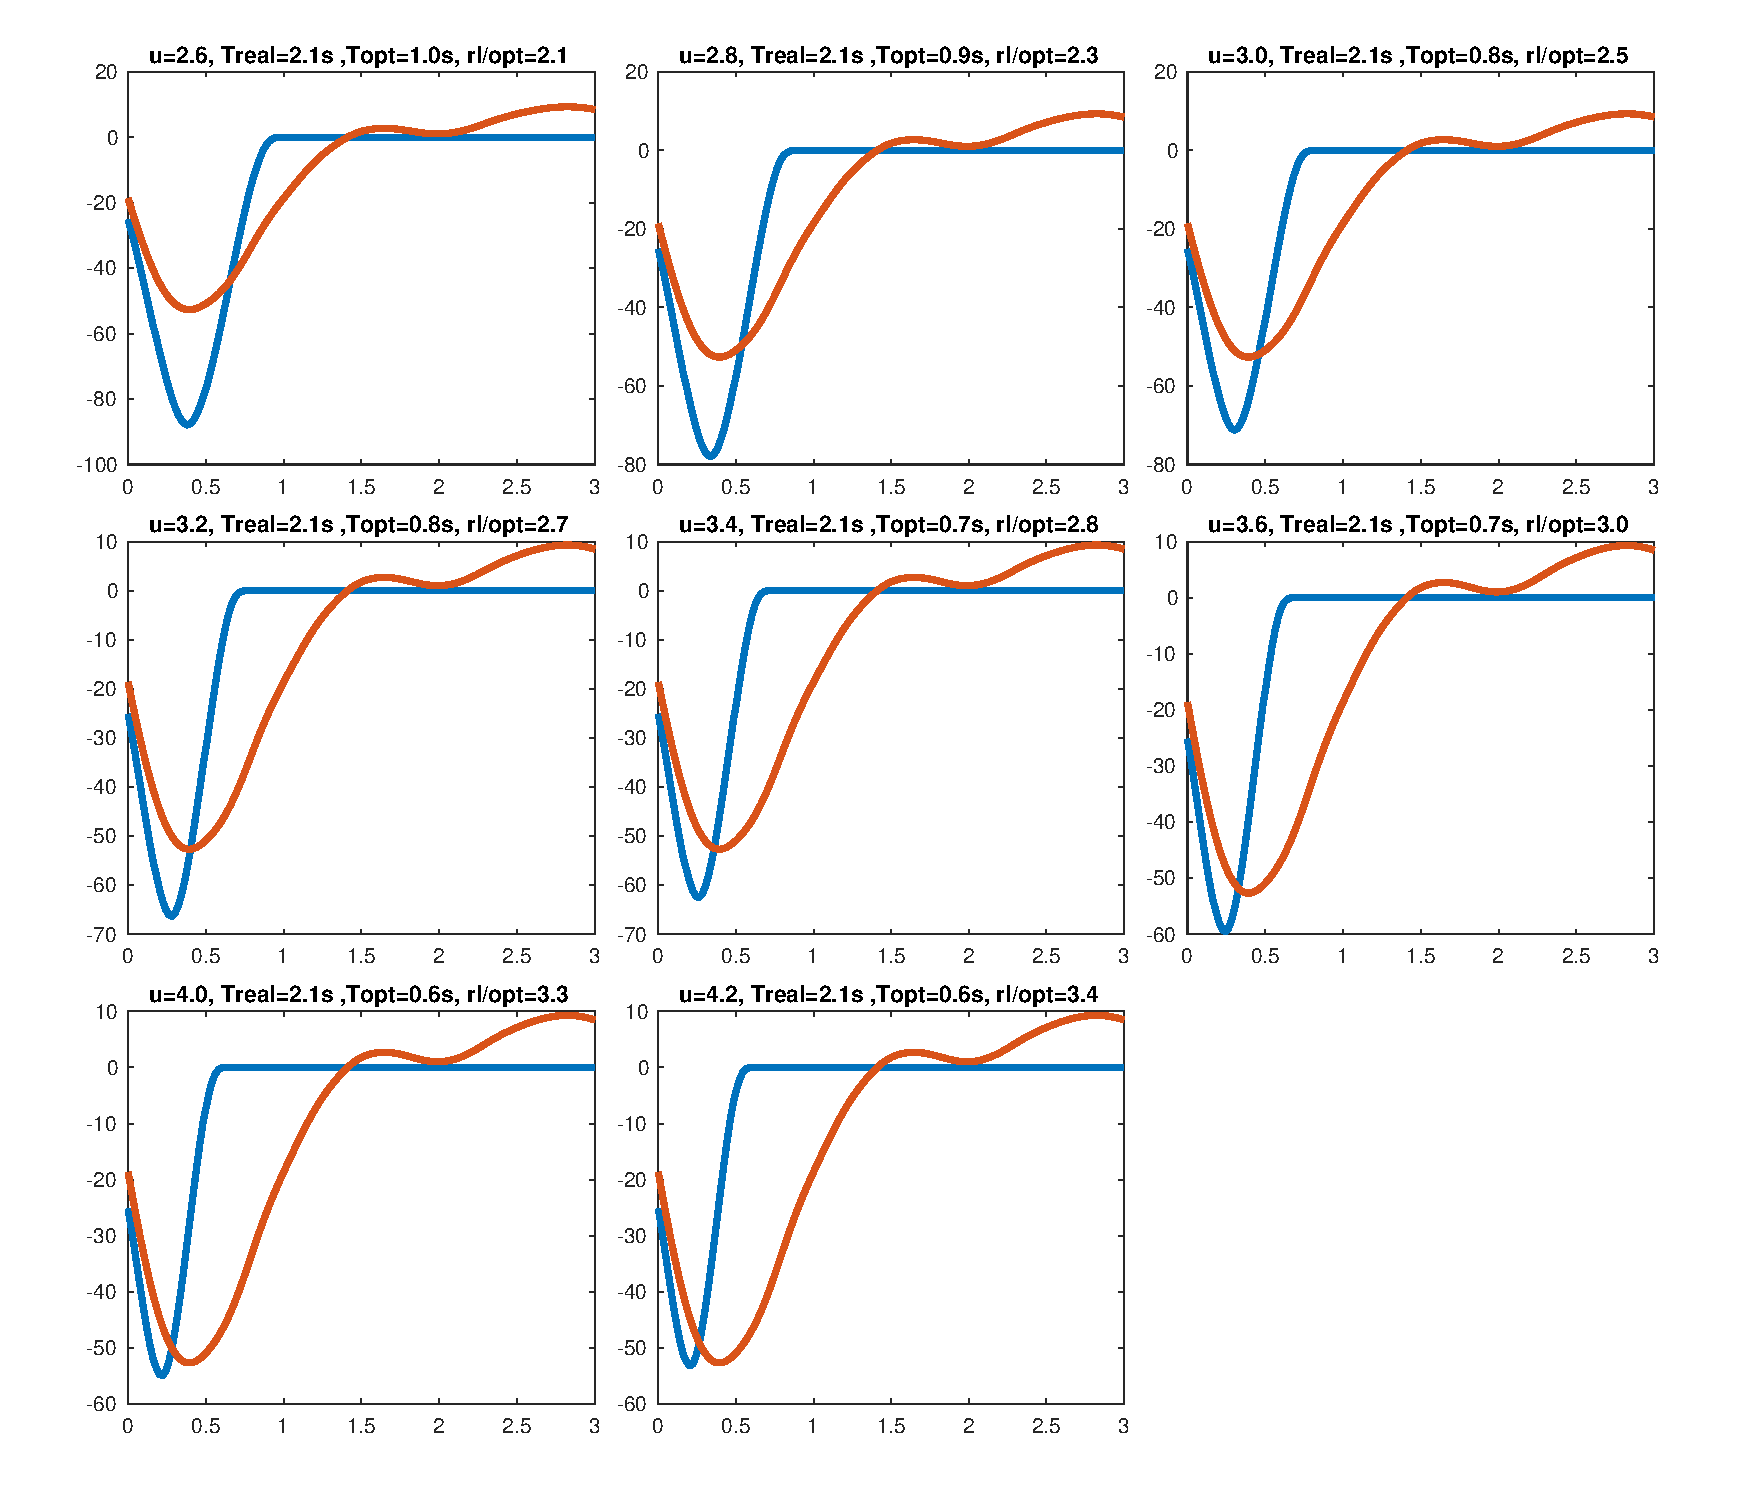
\includegraphics[width=1\linewidth]{final_graphs_1.eps}
    \caption{Сравнение характерных оптимальных(пунктирные) и реальных(сплошные) траектории на возвратном движении человека $t=1130$}
    \label{final_graphs_1}
\end{figure}

При таком управлении для нескольких толчков, максимальная амплитуда наиболее близка к реальной, поэтому для дальнейшего анализа будем рассматривать $u_*=3.2$ и $u_*=3.6$


Результаты аналогичного анализа для нескольких толчков,
представлены в таблице \ref{final_table}.

$F_{max} - $ максимальное значение силы с которой происходит толчок

$\varphi_0 - $ угол на который отклонился человек после заверешния толчка

$\omega_0 - $ угловая скорость, которую получил человек после завершения толчка

$\text{Момент } - $ момент в мышцах, возникший к моменту завершению толчка

$real/opt - $ отношение реального времени возврата к оптимальному при конкретном $u_\ast$

По ней видно, что среднее отношение реального времени завершения толчка к оптимальному равно 2.8 для сильных(номер $1-5$)
толчков и $1.86$ для слабых ($7-9$) при управлении $u_*=3.2$.


\begin{table}[h!]
    \centering
    \begin{tabular}{|l|c|c|c|c|c|c|c|c|c|}
        \hline
        \textbf{Номер толчка}       & \textbf{1} & \textbf{2} & \textbf{3} & \textbf{4} & \textbf{5} & \textbf{6} & \textbf{7} & \textbf{8} & \textbf{9} \\ \hline
        \textbf{$F_{max}$(Н)}       & 6.01       & 6.87       & 8.21       & 8.56       & 9.73       & 4.74       & 5.49       & 1.97       & 3.3        \\ \hline
        \textbf{Время толчка(сек)}  & 0.26       & 0.26       & 0.26       & 0.26       & 0.26       & 0.26       & 0.26       & 0.26       & 0.26       \\ \hline
        \textbf{$\varphi_0$ рад}        & 0.026      & 0.028      & 0.033      & 0.033      & 0.035      & 0.022      & 0.018      & 0.008      & 0.007      \\ \hline
        \textbf{$\omega_0$ рад/с}         & 0.15     & 0.18     & 0.17     & 0.20     & 0.21     & 0.10     & 0.15     & 0.05     & 0.08     \\ \hline
        \textbf{Момент(Н$\cdot$м)}       & 14.88      & 19.21      & 17.95      & 19.28      & 19.95      & 9.97       & 14.16      & 6.38       & 7.95       \\ \hline
        \textbf{real/opt $u_*=3.2$} & 2.8        & 2.7        & 2.8        & 2.8        & 2.9        & 2.7        & 1.8        & 1.8        & 2.0        \\ \hline
        \textbf{real/opt $u_*=3.6$} & 3.1        & 3.0        & 3.1        & 3.1        & 3.2        & 2.9        & 2.0        & 2.0        & 2.3        \\ \hline
    \end{tabular}
    \caption{Анализ различных толчков}
    \label{final_table}
\end{table}
\newpage
\section{Предолжения по корректировке и расширению задачи}

Результаты эксперимента совпадают с ожидаемым результатом: оптимальная траектория по форме совпадает с реальной,
 но при постановке оптимальной задачи были приняты излишне сильные допущения, в результате чего, оптимальная траектория отличается от реальной намного более быстрым временем возврата.
Видимо нервная система не успела среагировать, а среагировали камбаловидная или икроножная мышцы, их быстрореагирущие волокна.
За счет чего и успел возникнуть момент.

Ниже представлен список предложений, которые можно использовать для уточнения решения задачи:
\begin{enumerate}
    \item Считать, что после толчка момент в голеностопе уже успел измениться, что изменит начальные условия для задачи быстродействия 
    и потребует учета ненулевого значения момента в голеностопном суставе, что не предполагала исходная постановка задачи управления
    \item Использовать ДУСы, добавить видеозапись эксперимента для построения еще одной независиммой оценки начальных условий после толчка;
    \item Уточнить соответствие математической модели и физиологических способностей человека, для более детального описания процесса возврата;
    \item Набрать статистику: провести эксперимент на спортсменах, космонавтах, студентах и людях с проблемами опорно-двигательного аппарата.
\end{enumerate}


\newpage


\chapter*{Заключение}

\addcontentsline{toc}{chapter}{Заключение}

В дипломной работе решена задача оптимального управления,
 задача быстродействия, построенная с использованием принципа максимума Понтрягина.
 Представленный алгоритм позволяет определить оптимальную траекторию и время возвращения в исходную позу после толчка.
Тело человека моделировалось перевернутым маятником, как это традиционно принято в литераутре\cite{gurfincel}. Предполагалось, что такая постановка соответствует процессу восстановления позы после толчка.
В задаче ставилось ограничения на скорость изменения момента в голеностопном суставе.

Показано, что для данной задачи нет особых управлений, а регулярное принимает одинаковое по модулю значение, но чередуется по знаку, на различных участках движения. Решение задачи быстродействия сведено к нахождению корней полинома четвертой степени.

Для определения неизвестных параметров задачи использовались экспериментальные данные: показания саггитальной координаты центра давления, веса человека и показания силомера.
По данным центра давления с помощью метода двойной фильтрации восстанавливалсь траектория центра масс, а по ней находились начальные условия задачи быстродействия.
 С помощью анализа выборки толчков определялся максимальный момент, возникающий в голеностопном суставе.

Проведено сравнение рельной траектории процесса и оптимальной, показано, что качественно они совпадают, но за счет грубых, излишне приближенных начальных допущений, времена возврата в исходную позу сильно отличаются.


В ходе работы:
\begin{itemize}
    \item Показано, что решение оптимальной задачи быстродействия при ограниченной
          скорости изменения момента в голеностопном суставе может иметь решение, которое качественно совпадает с картиной, наблюдаемой в стабилометрических исследованиях;
    \item Представлено аналитическое решение задачи быстродействия;
    \item Найдены начальные условия в момент завершения толчка, с помощью метода двойной фильтрации;
    \item Время необходимое для восстановления исходной позы получилось
          соизмеримым с реальным времени возвращения после толчка;
    \item Проведен анализ допущений, которые могут скорректировать соответствие математической модели и реального процесса.
\end{itemize}





\newpage

\addcontentsline{toc}{chapter}{Литература}

\begin{thebibliography}{15}
    \bibitem{pandy}Pandy M.G., Zajac F.E., Sim E., Levine W.S. An optimal control model for maximum height human jumping// Journal of Biomechanics.-1990, vol. 23 – pp.1185-1198.
    \bibitem{humanMovements}Happee R. Time optimality in the control of human movements// Biological cybernetics- 1992, vol. 66 – pp. 357-366.
    \bibitem{AdaptFizkult}Слива С.С., Войнов И.Д., Слива А.С. Стабилоанализаторы в адаптивной физической культуре и спорте// IV Международная научная конференция по вопросам состояния и перспективам развития медицины в спорте высших достижений «СПОРТМЕД-2009» - М.: Экспоцентр, 2009.– С.121-123.
    \bibitem{pusher}Мельников А.А., Филёва В.В. Методика определения устойчивости вертикальной позы под влиянием внешнего толкающего воздействия // Физиология человека. 2015. С. 31–37.
    \bibitem{PAKrychinin}Кручинин П.А. Анализ результатов стабилометрических тестов со ступенчатым воздействием с точки зрения механики управляемых систем
    // Биофизика. – 2019. – Т. 64, №5. – С. 1–11.
    \bibitem{gurfincel}Гурфинкель В.С., Коц Я.М., Шик М.Л. Регуляция позы человека - М.: Наука, 1965 - 256 с.
    \bibitem{Optimal} Александров В.В., Лемак С.С., Парусников Н.А. Лекции по механике управляемых систем. Москва, Механико-математический факультет МГУ, 2020, 165 с.
    \bibitem{feldbaum}Фельдбаум А.А. Основы теории оптимальных автоматических систем. М.: Физматгиз, 1963. 552 с.
    \bibitem{kruchPodoprihin} П.А. Кручинин, М.А. Подоприхин, И.Д. Бекеров Cравнительный анализ алгоритмов оценки движения
    центра масс по результатам стабилометрических измерений // Биофизика. – 2021. – Т. 66, №5. – С. 997–1004.
    \bibitem{atansfalb}Фалб Питер Л., Атанс Майкл Оптимальное управление, Машиностроение, 1968, 764 с.
    \bibitem{kruchinMetoda} П.А. Кручинин Исследование колебаний человека при
    спокойном стоянии //Задача спецпрактикума по теоретической и прикладной механике. Изд-во мех.-мат. ф-та МГУ, 2022, 36 c.
    \bibitem{kozlovskay} Д. Г. Саенко, А. А. Артамонов, И. Б. Козловская Характеристики позных коррекционных ответов
    до и после длительных космических полетов // Физиология человека. – 2011. – Т. 37, №5. – С. 91–99.
\end{thebibliography}
\end{document}